\PassOptionsToPackage{unicode=true}{hyperref} % options for packages loaded elsewhere
\PassOptionsToPackage{hyphens}{url}
%
\documentclass[12pt,ignorenonframetext,aspectratio=169]{beamer}
\usepackage{pgfpages}
\setbeamertemplate{caption}[numbered]
\setbeamertemplate{caption label separator}{: }
\setbeamercolor{caption name}{fg=normal text.fg}
\beamertemplatenavigationsymbolsempty
% Prevent slide breaks in the middle of a paragraph:
\widowpenalties 1 10000
\raggedbottom
\setbeamertemplate{part page}{
\centering
\begin{beamercolorbox}[sep=16pt,center]{part title}
  \usebeamerfont{part title}\insertpart\par
\end{beamercolorbox}
}
\setbeamertemplate{section page}{
\centering
\begin{beamercolorbox}[sep=12pt,center]{part title}
  \usebeamerfont{section title}\insertsection\par
\end{beamercolorbox}
}
\setbeamertemplate{subsection page}{
\centering
\begin{beamercolorbox}[sep=8pt,center]{part title}
  \usebeamerfont{subsection title}\insertsubsection\par
\end{beamercolorbox}
}
\AtBeginPart{
  \frame{\partpage}
}
\AtBeginSection{
  \ifbibliography
  \else
    \frame{\sectionpage}
  \fi
}
\AtBeginSubsection{
  \frame{\subsectionpage}
}
\usepackage{lmodern}
\usepackage{amssymb,amsmath}
\usepackage{ifxetex,ifluatex}
\usepackage{fixltx2e} % provides \textsubscript
\ifnum 0\ifxetex 1\fi\ifluatex 1\fi=0 % if pdftex
  \usepackage[T1]{fontenc}
  \usepackage[utf8]{inputenc}
  \usepackage{textcomp} % provides euro and other symbols
\else % if luatex or xelatex
  \usepackage{unicode-math}
  \defaultfontfeatures{Ligatures=TeX,Scale=MatchLowercase}
\fi
\usetheme[]{metropolis}
% use upquote if available, for straight quotes in verbatim environments
\IfFileExists{upquote.sty}{\usepackage{upquote}}{}
% use microtype if available
\IfFileExists{microtype.sty}{%
\usepackage[]{microtype}
\UseMicrotypeSet[protrusion]{basicmath} % disable protrusion for tt fonts
}{}
\IfFileExists{parskip.sty}{%
\usepackage{parskip}
}{% else
\setlength{\parindent}{0pt}
\setlength{\parskip}{6pt plus 2pt minus 1pt}
}
\usepackage{hyperref}
\hypersetup{
            pdftitle={Computational Bayesian data analysis},
            pdfauthor={Bruno Nicenboim / Shravan Vasishth},
            pdfborder={0 0 0},
            breaklinks=true}
\urlstyle{same}  % don't use monospace font for urls
\newif\ifbibliography
\usepackage{color}
\usepackage{fancyvrb}
\newcommand{\VerbBar}{|}
\newcommand{\VERB}{\Verb[commandchars=\\\{\}]}
\DefineVerbatimEnvironment{Highlighting}{Verbatim}{commandchars=\\\{\}}
% Add ',fontsize=\small' for more characters per line
\usepackage{framed}
\definecolor{shadecolor}{RGB}{248,248,248}
\newenvironment{Shaded}{\begin{snugshade}}{\end{snugshade}}
\newcommand{\AlertTok}[1]{\textcolor[rgb]{0.94,0.16,0.16}{#1}}
\newcommand{\AnnotationTok}[1]{\textcolor[rgb]{0.56,0.35,0.01}{\textbf{\textit{#1}}}}
\newcommand{\AttributeTok}[1]{\textcolor[rgb]{0.77,0.63,0.00}{#1}}
\newcommand{\BaseNTok}[1]{\textcolor[rgb]{0.00,0.00,0.81}{#1}}
\newcommand{\BuiltInTok}[1]{#1}
\newcommand{\CharTok}[1]{\textcolor[rgb]{0.31,0.60,0.02}{#1}}
\newcommand{\CommentTok}[1]{\textcolor[rgb]{0.56,0.35,0.01}{\textit{#1}}}
\newcommand{\CommentVarTok}[1]{\textcolor[rgb]{0.56,0.35,0.01}{\textbf{\textit{#1}}}}
\newcommand{\ConstantTok}[1]{\textcolor[rgb]{0.00,0.00,0.00}{#1}}
\newcommand{\ControlFlowTok}[1]{\textcolor[rgb]{0.13,0.29,0.53}{\textbf{#1}}}
\newcommand{\DataTypeTok}[1]{\textcolor[rgb]{0.13,0.29,0.53}{#1}}
\newcommand{\DecValTok}[1]{\textcolor[rgb]{0.00,0.00,0.81}{#1}}
\newcommand{\DocumentationTok}[1]{\textcolor[rgb]{0.56,0.35,0.01}{\textbf{\textit{#1}}}}
\newcommand{\ErrorTok}[1]{\textcolor[rgb]{0.64,0.00,0.00}{\textbf{#1}}}
\newcommand{\ExtensionTok}[1]{#1}
\newcommand{\FloatTok}[1]{\textcolor[rgb]{0.00,0.00,0.81}{#1}}
\newcommand{\FunctionTok}[1]{\textcolor[rgb]{0.00,0.00,0.00}{#1}}
\newcommand{\ImportTok}[1]{#1}
\newcommand{\InformationTok}[1]{\textcolor[rgb]{0.56,0.35,0.01}{\textbf{\textit{#1}}}}
\newcommand{\KeywordTok}[1]{\textcolor[rgb]{0.13,0.29,0.53}{\textbf{#1}}}
\newcommand{\NormalTok}[1]{#1}
\newcommand{\OperatorTok}[1]{\textcolor[rgb]{0.81,0.36,0.00}{\textbf{#1}}}
\newcommand{\OtherTok}[1]{\textcolor[rgb]{0.56,0.35,0.01}{#1}}
\newcommand{\PreprocessorTok}[1]{\textcolor[rgb]{0.56,0.35,0.01}{\textit{#1}}}
\newcommand{\RegionMarkerTok}[1]{#1}
\newcommand{\SpecialCharTok}[1]{\textcolor[rgb]{0.00,0.00,0.00}{#1}}
\newcommand{\SpecialStringTok}[1]{\textcolor[rgb]{0.31,0.60,0.02}{#1}}
\newcommand{\StringTok}[1]{\textcolor[rgb]{0.31,0.60,0.02}{#1}}
\newcommand{\VariableTok}[1]{\textcolor[rgb]{0.00,0.00,0.00}{#1}}
\newcommand{\VerbatimStringTok}[1]{\textcolor[rgb]{0.31,0.60,0.02}{#1}}
\newcommand{\WarningTok}[1]{\textcolor[rgb]{0.56,0.35,0.01}{\textbf{\textit{#1}}}}
\usepackage{longtable,booktabs}
\usepackage{caption}
% These lines are needed to make table captions work with longtable:
\makeatletter
\def\fnum@table{\tablename~\thetable}
\makeatother
\usepackage{graphicx,grffile}
\makeatletter
\def\maxwidth{\ifdim\Gin@nat@width>\linewidth\linewidth\else\Gin@nat@width\fi}
\def\maxheight{\ifdim\Gin@nat@height>\textheight\textheight\else\Gin@nat@height\fi}
\makeatother
% Scale images if necessary, so that they will not overflow the page
% margins by default, and it is still possible to overwrite the defaults
% using explicit options in \includegraphics[width, height, ...]{}
\setkeys{Gin}{width=\maxwidth,height=\maxheight,keepaspectratio}
\setlength{\emergencystretch}{3em}  % prevent overfull lines
\providecommand{\tightlist}{%
  \setlength{\itemsep}{0pt}\setlength{\parskip}{0pt}}
\setcounter{secnumdepth}{5}

% set default figure placement to htbp
\makeatletter
\def\fps@figure{htbp}
\makeatother

  \setbeamercolor{frametitle}{bg=gray}
  \hypersetup{colorlinks,citecolor=orange,filecolor=red,linkcolor=brown,urlcolor=blue}
% \setsansfont[BoldFont={FiraSans-Bold.ttf}]{FiraSans-Light.ttf}
% \setmonofont{FiraMono-Regular.ttf}
\usepackage[sfdefault]{FiraSans}
\newcommand{\hideFromPandoc}[1]{#1}
         \hideFromPandoc{
             \let\Begin\begin
             \let\End\end
         }

\setbeamerfont{caption}{size=\scriptsize}

\title{Computational Bayesian data analysis}
\author{Bruno Nicenboim / Shravan Vasishth}
\date{2020-03-11}

\begin{document}
\frame{\titlepage}

\begin{frame}
\tableofcontents[hideallsubsections]
\end{frame}
\begin{frame}{}
\protect\hypertarget{section}{}

\begin{itemize}
\tightlist
\item
  Deriving the posterior distribution analytically is possible for only a very limited number of cases.
\item
  The denominator, the marginal likelihood, requires us to integrate the numerator:
\end{itemize}

\begin{equation}
p(\Theta|y) = \cfrac{ p(y|\Theta) \cdot p(\Theta) }{\int_{\Theta} p(y|\Theta) \cdot p(\Theta) d\Theta }
\end{equation}

\end{frame}

\begin{frame}{Alternative: Deriving the posterior through sampling}
\protect\hypertarget{alternative-deriving-the-posterior-through-sampling}{}

\small

\normalsize

\small

\normalsize

\small

\normalsize

\begin{block}{We want to derive the posterior distribution of the Cloze probability of \emph{``umbrella''}, \(\theta\):}

\begin{itemize}
\tightlist
\item
  Data: a word (e.g., \emph{``umbrella''}) was answered 80 out of 100 times,
\item
  Likelihood: a binomial distribution
\item
  Prior for \(\theta\): \(Beta(a=4,b=4)\)
\end{itemize}

\end{block}

\end{frame}

\begin{frame}

\begin{block}{We sample from the posterior distribution of \(\theta\):}

\begin{itemize}
\tightlist
\item
  We use a probabilistic programming language,
\item
  given enough samples we will have a good approximation of the real posterior distribution,
\item
  say we got 20000 samples from the posterior distribution of the Cloze probability, \(\theta\):
\end{itemize}

\scriptsize

0.712, 0.838, 0.767, 0.743, 0.732, 0.804, 0.738, 0.832, 0.851, 0.816, 0.771, 0.817, 0.721, 0.705, 0.827, 0.808, 0.776, 0.823, 0.786, 0.78, \ldots{}

\end{block}

\end{frame}

\begin{frame}

The approximation of the posterior looks quite similar to the real posterior.\footnote<.->{The difference between the true and the approximated mean and variance are 0.0002 and -0.00000003 respectively}



\small

\begin{figure}
\centering
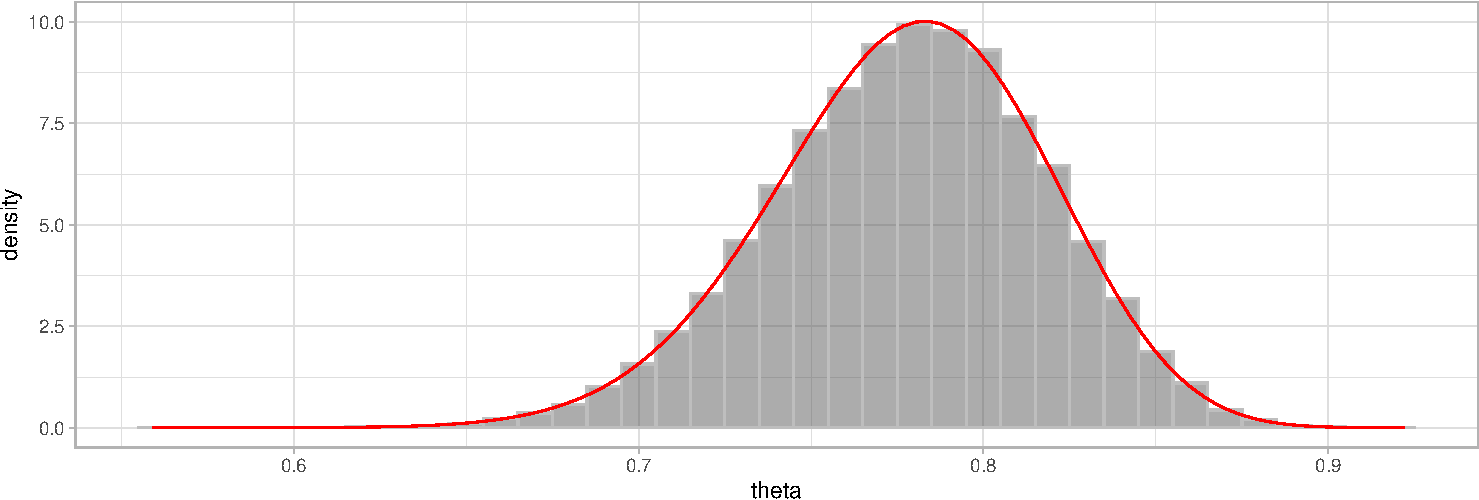
\includegraphics{03-compbayes-slides_files/figure-beamer/betapost-1.pdf}
\caption{\label{fig:betapost}Histogram of the samples of \(\theta\) from the posterior distribution calculated through sampling in gray; density plot of the exact posterior in red.}
\end{figure}

\normalsize

\end{frame}

\begin{frame}[fragile]{Computational Bayesian data analysis:}
\protect\hypertarget{computational-bayesian-data-analysis}{}

\begin{block}{Why now?}

\begin{itemize}
\tightlist
\item
  increase in computing power
\item
  appearance of probabilistic programming languages: WinBUGS (Lunn et al. 2000), JAGS (Plummer 2016), and more recently pymc3 (Salvatier, Wiecki, and Fonnesbeck 2016) and Stan (Carpenter et al. 2017).
\end{itemize}

\end{block}

\begin{block}{Easier alternatives based on Stan:}

\begin{itemize}
\tightlist
\item
  \texttt{rstanarm} (Goodrich et al. 2018)
\item
  \texttt{brms} (Bürkner 2019)
\end{itemize}

\end{block}

\end{frame}

\hypertarget{bayesian-regression-models-using-stan-brms}{%
\section{Bayesian Regression Models using `Stan': brms}\label{bayesian-regression-models-using-stan-brms}}

\begin{frame}[fragile]{Load the following:}
\protect\hypertarget{load-the-following}{}

\scriptsize

\begin{Shaded}
\begin{Highlighting}[]
\KeywordTok{set.seed}\NormalTok{(}\DecValTok{42}\NormalTok{)}
\KeywordTok{library}\NormalTok{(MASS)}
\CommentTok{## be careful to load dplyr after MASS}
\KeywordTok{library}\NormalTok{(dplyr)}
\KeywordTok{library}\NormalTok{(tidyr)}
\KeywordTok{library}\NormalTok{(purrr)}
\KeywordTok{library}\NormalTok{(readr)}
\KeywordTok{library}\NormalTok{(ggplot2)}
\KeywordTok{library}\NormalTok{(brms)}
\CommentTok{## Save compiled models:}
\KeywordTok{rstan_options}\NormalTok{(}\DataTypeTok{auto_write =} \OtherTok{TRUE}\NormalTok{)}
\CommentTok{## Parallelize the chains using all the cores:}
\KeywordTok{options}\NormalTok{(}\DataTypeTok{mc.cores =}\NormalTok{ parallel}\OperatorTok{::}\KeywordTok{detectCores}\NormalTok{())}
\KeywordTok{library}\NormalTok{(bayesplot)}
\KeywordTok{library}\NormalTok{(tictoc)}
\end{Highlighting}
\end{Shaded}

\normalsize

\end{frame}

\hypertarget{examples-1-a-single-participant-pressing-a-button-repeatedly-a-simple-linear-model}{%
\section{Examples 1: A single participant pressing a button repeatedly (A simple linear model)}\label{examples-1-a-single-participant-pressing-a-button-repeatedly-a-simple-linear-model}}

\begin{frame}

We have data from a participant repeatedly pressing the space bar as fast as possible, without paying attention to any stimuli.

\begin{block}{Data:}

reaction times in milliseconds in each trial

\end{block}

\begin{block}{Question:}

How long does it take to press a key when there is no decision involved?

\end{block}

\end{frame}

\begin{frame}

\begin{block}{Assumptions:}

\begin{enumerate}
\tightlist
\item
  There is a true underlying time, \(\mu\), that the participant needs to press the space bar.
\item
  There is some noise in this process.
\item
  The noise is normally distributed (this assumption is questionable given that reaction times are generally skewed; we fix this assumption later).
\end{enumerate}

\end{block}

\end{frame}

\begin{frame}{Formal model:}
\protect\hypertarget{formal-model}{}

\begin{block}{Likelihood for each observation \(n\):}

\begin{equation}
\begin{aligned}
rt_n \sim Normal(\mu, \sigma)
\end{aligned}
\label{eq:rtlik}
\end{equation}

\end{block}

\begin{block}{(Bad) priors:}

\begin{equation}
\begin{aligned}
\mu &\sim Uniform(0, 60000) \\
\sigma &\sim Uniform(0, 2000) 
\end{aligned}
\label{eq:rtpriors}
\end{equation}

\end{block}

\end{frame}

\begin{frame}[fragile]{Fitting the model}
\protect\hypertarget{fitting-the-model}{}

We'll first load the data from \texttt{data/button\_press.csv}:

\small

\begin{Shaded}
\begin{Highlighting}[]
\NormalTok{df_noreading_data <-}
\StringTok{  }\KeywordTok{read_csv}\NormalTok{(}\StringTok{"./data/button_press.csv"}\NormalTok{)}
\NormalTok{df_noreading_data}
\end{Highlighting}
\end{Shaded}

\begin{verbatim}
## # A tibble: 361 x 2
##      rt trialn
##   <dbl>  <dbl>
## 1   141      1
## 2   138      2
## 3   128      3
## 4   132      4
## 5   126      5
## # ... with 356 more rows
\end{verbatim}

\normalsize

\end{frame}

\begin{frame}[fragile]

\small

\begin{Shaded}
\begin{Highlighting}[]
\KeywordTok{ggplot}\NormalTok{(df_noreading_data, }\KeywordTok{aes}\NormalTok{(rt)) }\OperatorTok{+}
\StringTok{  }\KeywordTok{geom_density}\NormalTok{() }\OperatorTok{+}
\StringTok{  }\KeywordTok{ggtitle}\NormalTok{(}\StringTok{"Button-press data"}\NormalTok{)}
\end{Highlighting}
\end{Shaded}

\begin{figure}
\centering
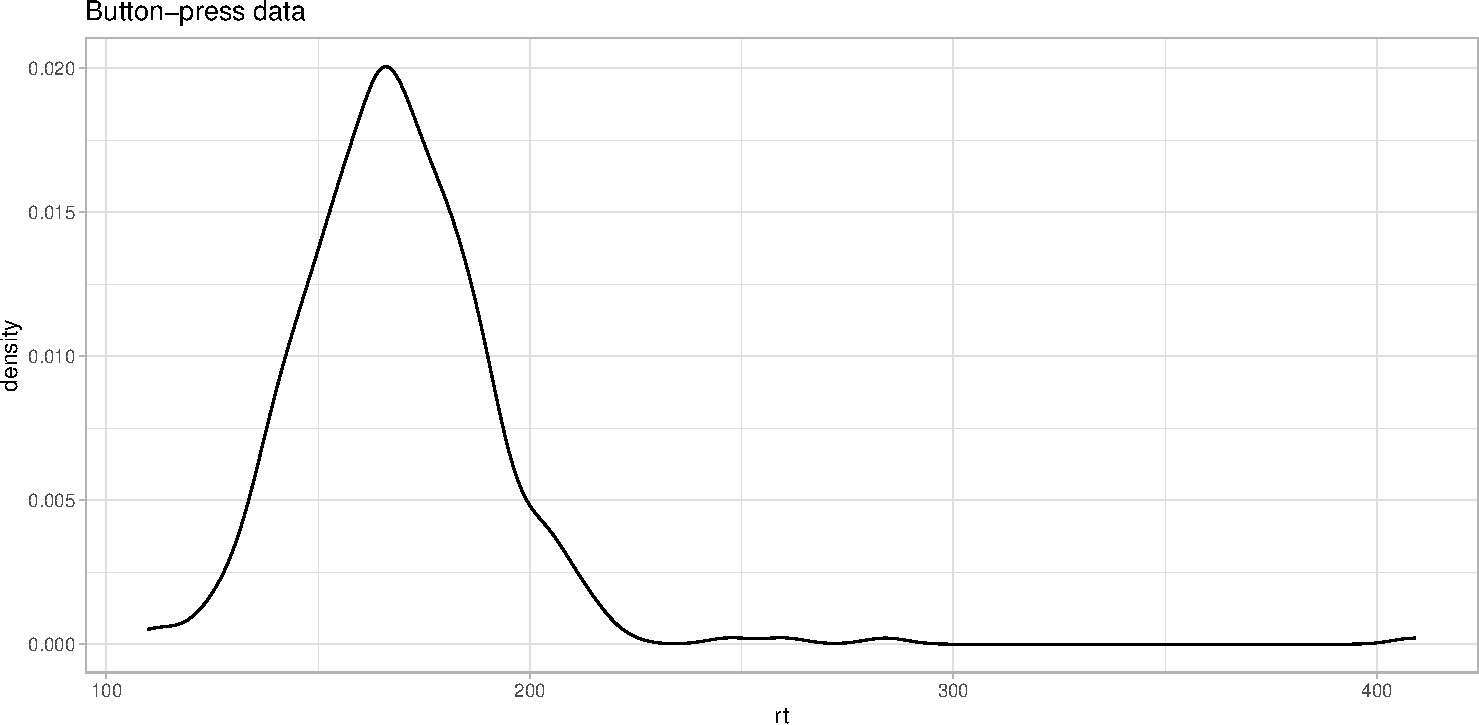
\includegraphics{03-compbayes-slides_files/figure-beamer/m1visualize-1.pdf}
\caption{\label{fig:m1visualize}Visualizing the data}
\end{figure}

\normalsize

\end{frame}

\begin{frame}[fragile]{Specifying the model in \texttt{brms}}
\protect\hypertarget{specifying-the-model-in-brms}{}

\small

\begin{Shaded}
\begin{Highlighting}[]
\NormalTok{fit_press <-}\StringTok{ }\KeywordTok{brm}\NormalTok{(rt }\OperatorTok{~}\StringTok{ }\DecValTok{1}\NormalTok{,}
  \DataTypeTok{data =}\NormalTok{ df_noreading_data,}
  \DataTypeTok{family =} \KeywordTok{gaussian}\NormalTok{(),}
  \DataTypeTok{prior =} \KeywordTok{c}\NormalTok{(}
    \KeywordTok{prior}\NormalTok{(}\KeywordTok{uniform}\NormalTok{(}\DecValTok{0}\NormalTok{, }\DecValTok{60000}\NormalTok{), }\DataTypeTok{class =}\NormalTok{ Intercept),}
    \KeywordTok{prior}\NormalTok{(}\KeywordTok{uniform}\NormalTok{(}\DecValTok{0}\NormalTok{, }\DecValTok{2000}\NormalTok{), }\DataTypeTok{class =}\NormalTok{ sigma)}
\NormalTok{  ),}
  \DataTypeTok{chains =} \DecValTok{4}\NormalTok{,}
  \DataTypeTok{iter =} \DecValTok{2000}\NormalTok{,}
  \DataTypeTok{warmup =} \DecValTok{1000}
\NormalTok{)}
\end{Highlighting}
\end{Shaded}

\normalsize

\end{frame}

\begin{frame}[fragile]{Sampling and convergence in a nutshell}
\protect\hypertarget{sampling-and-convergence-in-a-nutshell}{}

\scriptsize

\begin{enumerate}
\tightlist
\item
  Chains start in random locations;
\item
  in each iteration they take one sample each;
\item
  samples at the beginning do not belong to the posterior distribution;
\item
  eventually, the chains end up in the vicinity of the posterior distribution;
\item
  from that point onwards the samples will belong to the posterior.
\end{enumerate}



\small

\begin{figure}
\centering
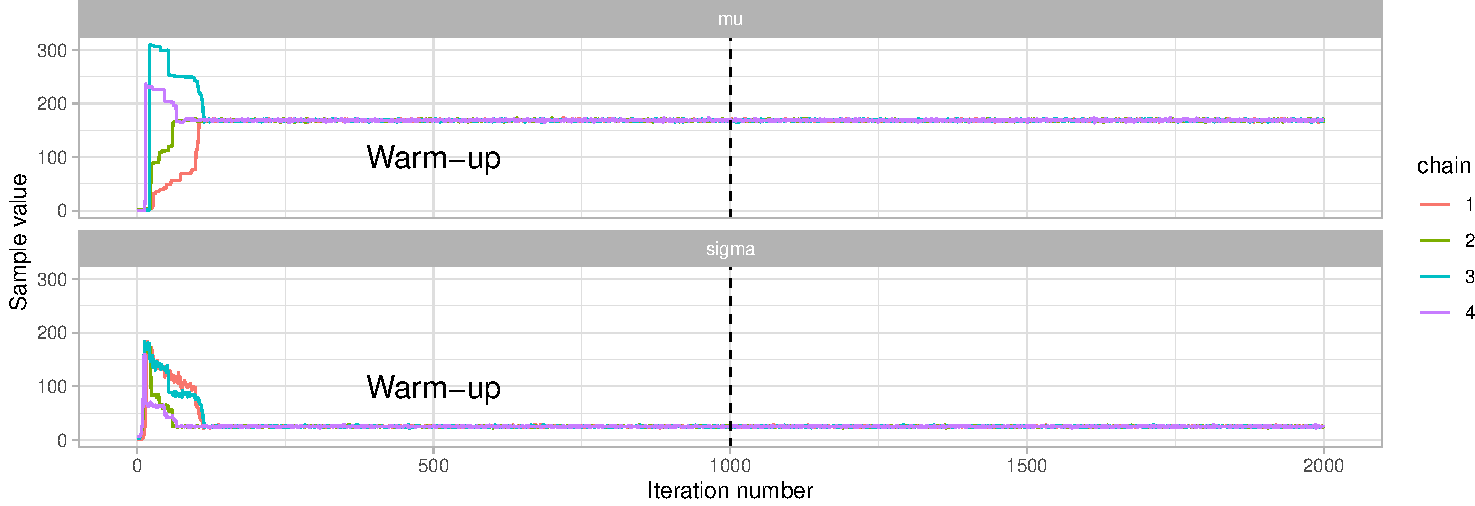
\includegraphics{03-compbayes-slides_files/figure-beamer/warmup-1.pdf}
\caption{\label{fig:warmup}Trace plot of the \texttt{brms} model}
\end{figure}

\normalsize

\end{frame}

\begin{frame}



\small

\begin{figure}
\centering
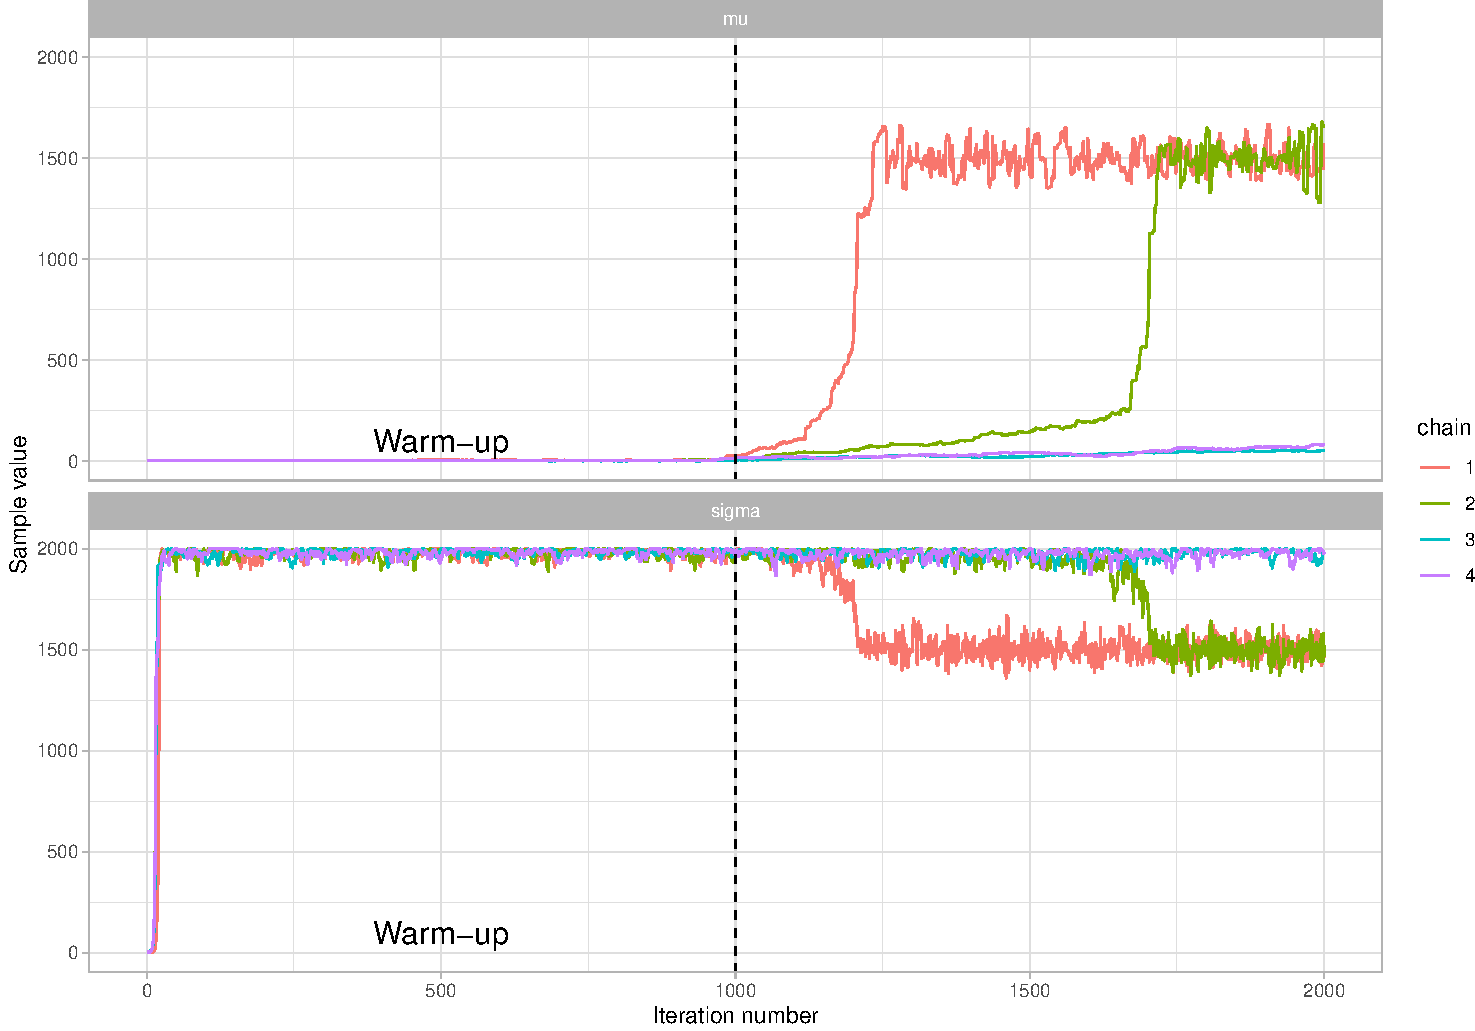
\includegraphics{03-compbayes-slides_files/figure-beamer/warmup2-1.pdf}
\caption{\label{fig:warmup2}Trace plot of a model that \textbf{did not} converge.}
\end{figure}

\normalsize

\end{frame}

\begin{frame}[fragile]{Output of \texttt{brms}}
\protect\hypertarget{output-of-brms}{}

\small

\begin{Shaded}
\begin{Highlighting}[]
\KeywordTok{posterior_samples}\NormalTok{(fit_press) }\OperatorTok\StringTok{ }\KeywordTok{str}\NormalTok{()}
\end{Highlighting}
\end{Shaded}

\begin{verbatim}
## 'data.frame':    4000 obs. of  3 variables:
##  $ b_Intercept: num  167 168 171 171 168 ...
##  $ sigma      : num  24.9 25.2 24.3 23.6 25.2 ...
##  $ lp__       : num  -1688 -1688 -1690 -1690 -1688 ...
\end{verbatim}

\normalsize

\end{frame}

\begin{frame}[fragile]{Output of \texttt{brms}}
\protect\hypertarget{output-of-brms-1}{}

\small

\begin{Shaded}
\begin{Highlighting}[]
\KeywordTok{plot}\NormalTok{(fit_press)}
\end{Highlighting}
\end{Shaded}

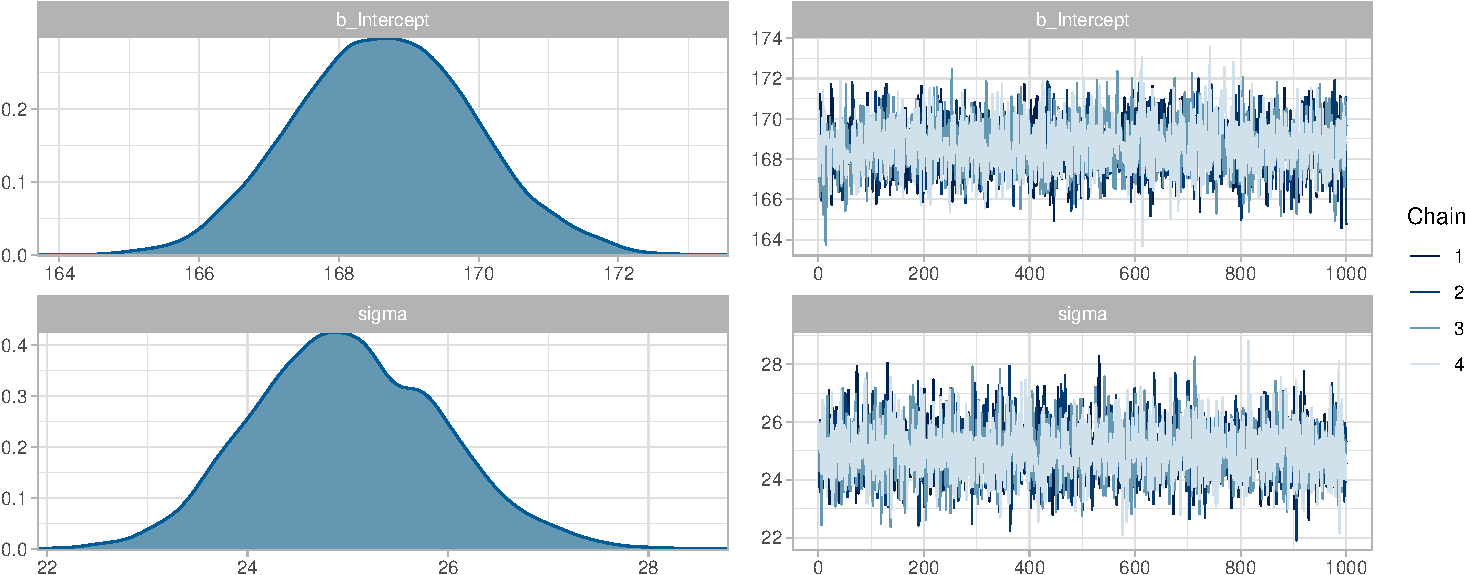
\includegraphics{03-compbayes-slides_files/figure-beamer/unnamed-chunk-5-1.pdf}

\normalsize

\end{frame}

\begin{frame}[fragile]{Output of \texttt{brms}}
\protect\hypertarget{output-of-brms-2}{}

\scriptsize

\begin{Shaded}
\begin{Highlighting}[]
\NormalTok{fit_press}
\CommentTok{# posterior_summary(fit_press) is also useful}
\end{Highlighting}
\end{Shaded}

\begin{verbatim}
##  Family: gaussian 
##   Links: mu = identity; sigma = identity 
## Formula: rt ~ 1 
##    Data: df_noreading_data (Number of observations: 361) 
## Samples: 4 chains, each with iter = 2000; warmup = 1000; thin = 1;
##          total post-warmup samples = 4000
## 
## Population-Level Effects: 
##           Estimate Est.Error l-95% CI u-95% CI Rhat
## Intercept   168.66      1.28   166.24   171.20 1.00
##           Bulk_ESS Tail_ESS
## Intercept     3295     2654
## 
## Family Specific Parameters: 
##       Estimate Est.Error l-95% CI u-95% CI Rhat
## sigma    25.00      0.93    23.26    26.91 1.00
##       Bulk_ESS Tail_ESS
## sigma     4184     2769
## 
## Samples were drawn using sampling(NUTS). For each parameter, Bulk_ESS
## and Tail_ESS are effective sample size measures, and Rhat is the potential
## scale reduction factor on split chains (at convergence, Rhat = 1).
\end{verbatim}

\normalsize

\end{frame}

\begin{frame}[fragile]{Output of \texttt{brms}}
\protect\hypertarget{output-of-brms-3}{}

Notice that the \texttt{Estimate} is just the mean of the posterior sample, and
CI are the 95\% quantiles:

\small

\begin{Shaded}
\begin{Highlighting}[]
\KeywordTok{posterior_samples}\NormalTok{(fit_press)}\OperatorTok{$}\NormalTok{b_Intercept }\OperatorTok
\StringTok{  }\KeywordTok{mean}\NormalTok{()}
\end{Highlighting}
\end{Shaded}

\begin{verbatim}
## [1] 169
\end{verbatim}

\begin{Shaded}
\begin{Highlighting}[]
\KeywordTok{posterior_samples}\NormalTok{(fit_press)}\OperatorTok{$}\NormalTok{b_Intercept }\OperatorTok
\StringTok{  }\KeywordTok{quantile}\NormalTok{(}\KeywordTok{c}\NormalTok{(}\FloatTok{0.025}\NormalTok{, }\FloatTok{.975}\NormalTok{))}
\end{Highlighting}
\end{Shaded}

\begin{verbatim}
## 2.5%  98% 
##  166  171
\end{verbatim}

\normalsize

\end{frame}

\begin{frame}

\begin{block}{\color{blue} Exercises}

3.8.1.1 Fit the model fit\_press with just a few of iterations? What happens?

3.8.1.2 Using uniform distributions, choose priors that represent better your assumptions about reaction times. What happens with the new model?

\end{block}

\end{frame}

\begin{frame}{Important questions}
\protect\hypertarget{important-questions}{}

\large

\begin{enumerate}
\tightlist
\item
  What information are the priors encoding? Do the priors make sense?
\item
  Does the likelihood assumed in the model make sense for the data?
\end{enumerate}

\end{frame}

\hypertarget{sec:priorpred}{%
\section{Prior predictive distributions}\label{sec:priorpred}}

We had defined the following priors for our linear model:

\begin{equation}
\begin{aligned}
\mu &\sim Uniform(0, 60000) \\
\sigma &\sim Uniform(0, 2000) 
\end{aligned}
\label{eq:rtpriorsrepeated}
\end{equation}

These priors encode assumptions about the kind of data we would expect to see in a future study.

Do the priors generate realistic-looking data?

\begin{frame}{Prior predictive distributions}
\protect\hypertarget{prior-predictive-distributions}{}

We want to know the density \(p(\cdot)\) of data points \(y_1,\dots,n\), given a vector of priors \(\Theta\) (e.g., \(\Theta=\langle\mu,\sigma \rangle\))

The prior predictive density is:

\begin{equation}
p(y_1,\dots,y_n)= \int p(y|\Theta)\cdot p(y_2|\Theta)\cdots p(y_n|\Theta) p(\Theta) \, d\Theta 
\end{equation}

We avoid doing the integration by generating samples from the prior distribution. We repeat the following:

\begin{enumerate}
\tightlist
\item
  Take one sample from each of the priors.
\item
  Plug those samples in the likelihood and generate a dataset \(y_{pred_1},\ldots,y_{pred_n}\).
\end{enumerate}

\end{frame}

\begin{frame}[fragile]

\vspace{.1in}

\scriptsize

\begin{Shaded}
\begin{Highlighting}[]
\NormalTok{normal_predictive_distribution <-}\StringTok{ }\ControlFlowTok{function}\NormalTok{(mu_samples, sigma_samples, N_obs) \{}
  \CommentTok{# empty data frame with headers:}
\NormalTok{  df_pred <-}\StringTok{ }\KeywordTok{tibble}\NormalTok{(}
    \DataTypeTok{trialn =} \KeywordTok{numeric}\NormalTok{(}\DecValTok{0}\NormalTok{),}
    \DataTypeTok{rt_pred =} \KeywordTok{numeric}\NormalTok{(}\DecValTok{0}\NormalTok{),}
    \DataTypeTok{iter =} \KeywordTok{numeric}\NormalTok{(}\DecValTok{0}\NormalTok{)}
\NormalTok{  )}
  \CommentTok{# i iterates from 1 to the length of mu_samples,}
  \CommentTok{# which we assume is identical to}
  \CommentTok{# the length of the sigma_samples:}
  \ControlFlowTok{for}\NormalTok{ (i }\ControlFlowTok{in} \KeywordTok{seq_along}\NormalTok{(mu_samples)) \{}
\NormalTok{    mu <-}\StringTok{ }\NormalTok{mu_samples[i]}
\NormalTok{    sigma <-}\StringTok{ }\NormalTok{sigma_samples[i]}
\NormalTok{    df_pred <-}\StringTok{ }\KeywordTok{bind_rows}\NormalTok{(}
\NormalTok{      df_pred,}
      \KeywordTok{tibble}\NormalTok{(}
        \DataTypeTok{trialn =} \KeywordTok{seq_len}\NormalTok{(N_obs), }\CommentTok{# 1, 2,... N_obs}
        \DataTypeTok{rt_pred =} \KeywordTok{rnorm}\NormalTok{(N_obs, mu, sigma),}
        \DataTypeTok{iter =}\NormalTok{ i}
\NormalTok{      )}
\NormalTok{    )}
\NormalTok{  \}}
\NormalTok{  df_pred}
\NormalTok{\}}
\end{Highlighting}
\end{Shaded}

\normalsize

\end{frame}

\begin{frame}[fragile]

This approach works, but it's quite slow:

\scriptsize

\begin{Shaded}
\begin{Highlighting}[]
\KeywordTok{tic}\NormalTok{()}
\NormalTok{N_samples <-}\StringTok{ }\DecValTok{1000}
\NormalTok{N_obs <-}\StringTok{ }\KeywordTok{nrow}\NormalTok{(df_noreading_data)}
\NormalTok{mu_samples <-}\StringTok{ }\KeywordTok{runif}\NormalTok{(N_samples, }\DecValTok{0}\NormalTok{, }\DecValTok{60000}\NormalTok{)}
\NormalTok{sigma_samples <-}\StringTok{ }\KeywordTok{runif}\NormalTok{(N_samples, }\DecValTok{0}\NormalTok{, }\DecValTok{2000}\NormalTok{)}
\KeywordTok{normal_predictive_distribution}\NormalTok{(}\DataTypeTok{mu_samples =}\NormalTok{ mu_samples,}
                               \DataTypeTok{sigma_samples =}\NormalTok{ sigma_samples,}
                                \DataTypeTok{N_obs =}\NormalTok{ N_obs)}
\KeywordTok{toc}\NormalTok{()}
\end{Highlighting}
\end{Shaded}

\begin{verbatim}
## # A tibble: 361,000 x 3
##   trialn rt_pred  iter
##    <dbl>   <dbl> <dbl>
## 1      1  44587.     1
## 2      2  48271.     1
## 3      3  50291.     1
## 4      4  48784.     1
## 5      5  49350.     1
## # ... with 3.61e+05 more rows
## 3.711 sec elapsed
\end{verbatim}

\normalsize

\end{frame}

\begin{frame}[fragile]

A more efficient version:

\scriptsize

\begin{Shaded}
\begin{Highlighting}[]
\NormalTok{normal_predictive_distribution_fast <-}\StringTok{ }\ControlFlowTok{function}\NormalTok{(mu_samples,}
\NormalTok{                                                sigma_samples,}
\NormalTok{                                                N_obs) \{}
  \CommentTok{# map_dfr works similarly to lapply, it essentially runs}
  \CommentTok{# a for-loop, and builds a dataframe with the output.}
  \CommentTok{# We iterate over the values of mu_samples and sigma_samples}
  \CommentTok{# simultaneously, and in each iteration we bind a new}
  \CommentTok{# data frame with N_obs observations.}
  \KeywordTok{map2_dfr}\NormalTok{(mu_samples, sigma_samples, }\ControlFlowTok{function}\NormalTok{(mu, sigma) \{}
    \KeywordTok{tibble}\NormalTok{(}
      \DataTypeTok{trialn =} \KeywordTok{seq_len}\NormalTok{(N_obs),}
      \DataTypeTok{rt_pred =} \KeywordTok{rnorm}\NormalTok{(N_obs, mu, sigma)}
\NormalTok{    )\}, }\DataTypeTok{.id =} \StringTok{"iter"}\NormalTok{) }\OperatorTok
\StringTok{    }\CommentTok{# .id is always a string and needs to be converted to a number}
\StringTok{    }\KeywordTok{mutate}\NormalTok{(}\DataTypeTok{iter =} \KeywordTok{as.numeric}\NormalTok{(iter))}
\NormalTok{\}}
\end{Highlighting}
\end{Shaded}

\normalsize

\end{frame}

\begin{frame}[fragile]

\scriptsize

\begin{Shaded}
\begin{Highlighting}[]
\KeywordTok{tic}\NormalTok{()}
\NormalTok{(prior_pred <-}\StringTok{ }\KeywordTok{normal_predictive_distribution_fast}\NormalTok{(}
  \DataTypeTok{mu_samples =}\NormalTok{ mu_samples,}
  \DataTypeTok{sigma_samples =}\NormalTok{ sigma_samples,}
\NormalTok{  N_obs))}
\KeywordTok{toc}\NormalTok{()}
\end{Highlighting}
\end{Shaded}

\begin{verbatim}
## # A tibble: 361,000 x 3
##    iter trialn rt_pred
##   <dbl>  <int>   <dbl>
## 1     1      1  48513.
## 2     1      2  46243.
## 3     1      3  48812.
## 4     1      4  49650.
## 5     1      5  49096.
## # ... with 3.61e+05 more rows
## 0.339 sec elapsed
\end{verbatim}

\normalsize

\end{frame}

\begin{frame}[fragile]

\vspace{.1in}



\scriptsize

\begin{Shaded}
\begin{Highlighting}[]
\NormalTok{prior_pred }\OperatorTok
\StringTok{  }\KeywordTok{filter}\NormalTok{(iter }\OperatorTok{<=}\StringTok{ }\DecValTok{12}\NormalTok{) }\OperatorTok
\StringTok{  }\KeywordTok{ggplot}\NormalTok{(}\KeywordTok{aes}\NormalTok{(rt_pred)) }\OperatorTok{+}
\StringTok{  }\KeywordTok{geom_histogram}\NormalTok{() }\OperatorTok{+}
\StringTok{  }\KeywordTok{facet_wrap}\NormalTok{(}\OperatorTok{~}\NormalTok{iter, }\DataTypeTok{ncol =} \DecValTok{3}\NormalTok{)}
\end{Highlighting}
\end{Shaded}

\begin{figure}
\centering
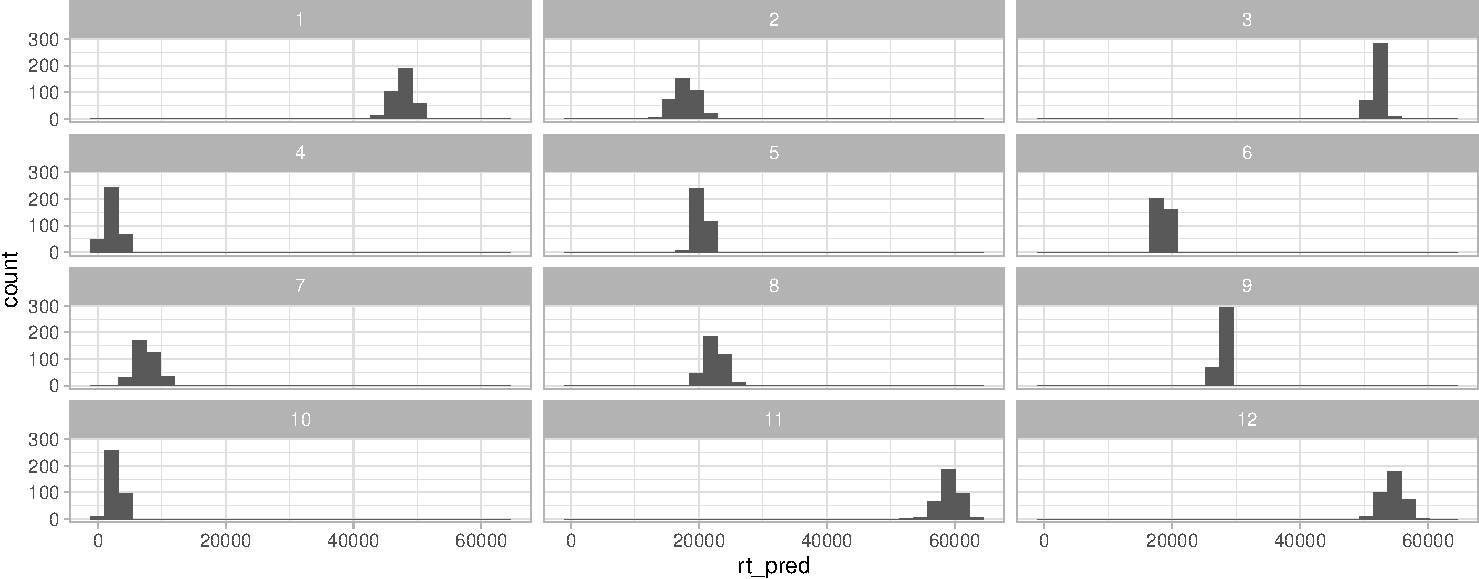
\includegraphics{03-compbayes-slides_files/figure-beamer/priorpred-simple-1.pdf}
\caption{\label{fig:priorpred-simple}Eighteen samples from the prior predictive distribution.}
\end{figure}

\normalsize

\end{frame}

\begin{frame}[fragile]{Distribution of statistics}
\protect\hypertarget{distribution-of-statistics}{}

\vspace{.1in}

\scriptsize

\begin{Shaded}
\begin{Highlighting}[]
\NormalTok{(prior_stat <-}\StringTok{ }\NormalTok{prior_pred }\OperatorTok
\StringTok{  }\KeywordTok{group_by}\NormalTok{(iter) }\OperatorTok
\StringTok{  }\KeywordTok{summarize}\NormalTok{(}\DataTypeTok{min_rt =} \KeywordTok{min}\NormalTok{(rt_pred),}
            \DataTypeTok{max_rt =} \KeywordTok{max}\NormalTok{(rt_pred),}
            \DataTypeTok{average_rt =} \KeywordTok{mean}\NormalTok{(rt_pred)) }\OperatorTok
\StringTok{  }\CommentTok{# we convert the previous data frame to a long one,}
\StringTok{  }\CommentTok{# where min_rt, max_rt, average_rt are possible values}
\StringTok{  }\CommentTok{# of the columns "stat"}
\StringTok{  }\KeywordTok{pivot_longer}\NormalTok{(}\DataTypeTok{cols =} \KeywordTok{ends_with}\NormalTok{(}\StringTok{"rt"}\NormalTok{),}
               \DataTypeTok{names_to =} \StringTok{"stat"}\NormalTok{,}
               \DataTypeTok{values_to =} \StringTok{"rt"}\NormalTok{))}
\end{Highlighting}
\end{Shaded}

\begin{verbatim}
## # A tibble: 3,000 x 3
##    iter stat           rt
##   <dbl> <chr>       <dbl>
## 1     1 min_rt     43017.
## 2     1 max_rt     52560.
## 3     1 average_rt 47753.
## 4     2 min_rt     13331.
## 5     2 max_rt     23830.
## # ... with 2,995 more rows
\end{verbatim}

\normalsize

\end{frame}

\begin{frame}[fragile]



\scriptsize

\begin{Shaded}
\begin{Highlighting}[]
\NormalTok{prior_stat }\OperatorTok
\StringTok{  }\KeywordTok{ggplot}\NormalTok{(}\KeywordTok{aes}\NormalTok{(rt)) }\OperatorTok{+}
\StringTok{  }\KeywordTok{geom_histogram}\NormalTok{(}\DataTypeTok{binwidth =} \DecValTok{500}\NormalTok{) }\OperatorTok{+}
\StringTok{  }\KeywordTok{facet_wrap}\NormalTok{(}\OperatorTok{~}\NormalTok{stat, }\DataTypeTok{ncol =} \DecValTok{1}\NormalTok{)}
\end{Highlighting}
\end{Shaded}

\begin{figure}
\centering
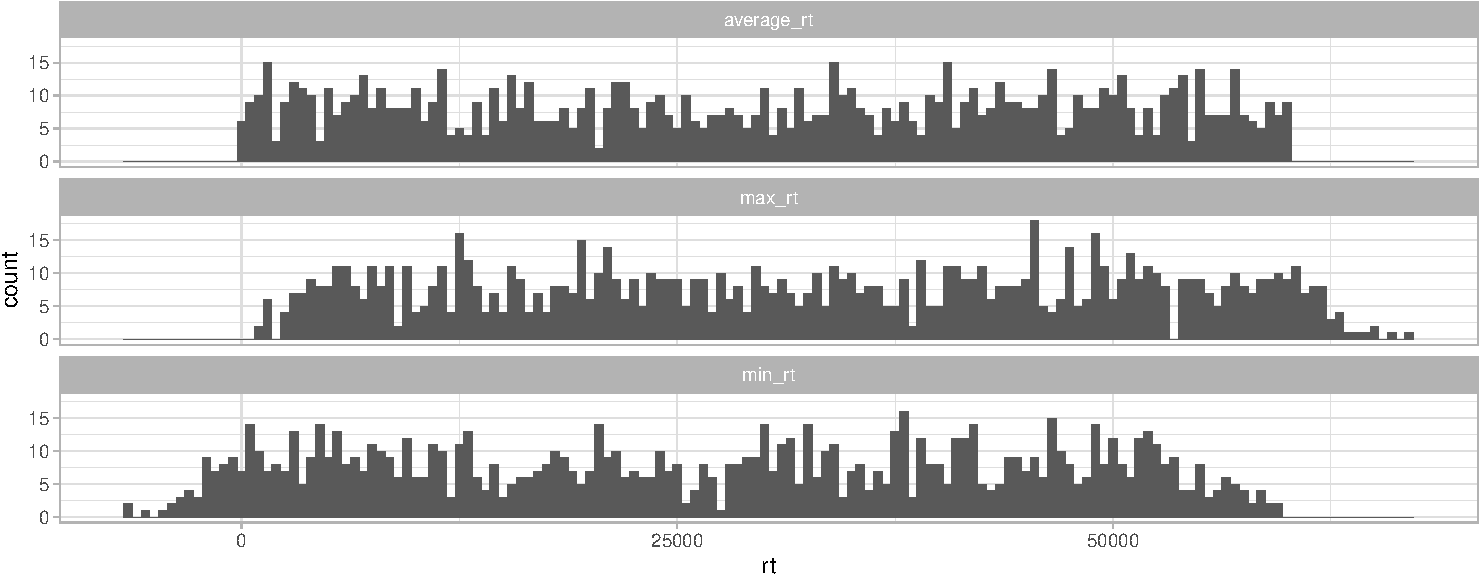
\includegraphics{03-compbayes-slides_files/figure-beamer/priorpred-stats-1.pdf}
\caption{\label{fig:priorpred-stats}Prior predictive distribution of averages, maximum, and minimum values.}
\end{figure}

\normalsize

\end{frame}

\begin{frame}

\begin{block}{Why are our distributions so bad?}

We used much less prior information than what we really had: our priors are clearly not very realistic given what we know about reaction times for such a button pressing task.

\end{block}

\begin{block}{What priors should we have chosen?}

\end{block}

\end{frame}

\hypertarget{sec:sensitivity}{%
\section{The influence of priors: sensitivity analysis}\label{sec:sensitivity}}

\begin{frame}{Types of priors}
\protect\hypertarget{types-of-priors}{}

\begin{enumerate}
\item
  \textbf{Flat uninformative priors}: priors as uninformative as possible. 
\item
  \textbf{Regularizing priors}: priors that downweight extreme values (that is, they provide regularization), they are not very informative, and mostly let the likelihood dominate in determining the posteriors. 
\item
  \textbf{Principled priors}: priors that encode all (or most of) the theory-neutral information that we do have. 
\item
  \textbf{Informative priors}: There are cases where we have a lot of prior knowledge, and not much data. 
\end{enumerate}

\end{frame}

\begin{frame}[fragile]{Revisiting the button-pressing example with different priors}
\protect\hypertarget{revisiting-the-button-pressing-example-with-different-priors}{}

What would happen if we use even wider priors for the model?

\begin{equation}
\begin{aligned}
\mu &\sim Uniform(-10^{10}, 10^{10}) \\
\sigma &\sim Uniform(0,  10^{10}) 
\end{aligned}
\label{eq:rtpriorsflat}
\end{equation}

\begin{block}{In brms:}

\small

\begin{Shaded}
\begin{Highlighting}[]
\NormalTok{fit_press_unif <-}\StringTok{ }\KeywordTok{brm}\NormalTok{(rt }\OperatorTok{~}\StringTok{ }\DecValTok{1}\NormalTok{,}
  \DataTypeTok{data =}\NormalTok{ df_noreading_data,}
  \DataTypeTok{family =} \KeywordTok{gaussian}\NormalTok{(),}
  \DataTypeTok{prior =} \KeywordTok{c}\NormalTok{(}
      \KeywordTok{prior}\NormalTok{(}\KeywordTok{uniform}\NormalTok{(}\OperatorTok{-}\DecValTok{10}\OperatorTok{^}\DecValTok{10}\NormalTok{, }\DecValTok{10}\OperatorTok{^}\DecValTok{10}\NormalTok{), }\DataTypeTok{class =}\NormalTok{ Intercept),}
    \KeywordTok{prior}\NormalTok{(}\KeywordTok{uniform}\NormalTok{(}\DecValTok{0}\NormalTok{, }\DecValTok{10}\OperatorTok{^}\DecValTok{10}\NormalTok{), }\DataTypeTok{class =}\NormalTok{ sigma))}
\NormalTok{)}
\end{Highlighting}
\end{Shaded}

\normalsize

\end{block}

\end{frame}

\begin{frame}[fragile]

The output of the model is virtually identical!

\scriptsize

\begin{Shaded}
\begin{Highlighting}[]
\NormalTok{fit_press_unif}
\end{Highlighting}
\end{Shaded}

\begin{verbatim}
##  Family: gaussian 
##   Links: mu = identity; sigma = identity 
## Formula: rt ~ 1 
##    Data: df_noreading_data (Number of observations: 361) 
## Samples: 4 chains, each with iter = 2000; warmup = 1000; thin = 1;
##          total post-warmup samples = 4000
## 
## Population-Level Effects: 
##           Estimate Est.Error l-95% CI u-95% CI Rhat
## Intercept   168.66      1.33   165.98   171.22 1.00
##           Bulk_ESS Tail_ESS
## Intercept     3155     2617
## 
## Family Specific Parameters: 
##       Estimate Est.Error l-95% CI u-95% CI Rhat
## sigma    24.99      0.94    23.27    26.90 1.00
##       Bulk_ESS Tail_ESS
## sigma     3652     2777
## 
## Samples were drawn using sampling(NUTS). For each parameter, Bulk_ESS
## and Tail_ESS are effective sample size measures, and Rhat is the potential
## scale reduction factor on split chains (at convergence, Rhat = 1).
\end{verbatim}

\normalsize

\end{frame}

\begin{frame}[fragile]

\begin{block}{What happens if we use very informative priors and they are off?}

\begin{equation}
\begin{aligned}
\mu &\sim Normal(400, 10) \\
\sigma &\sim Normal_+(100, 10) 
\end{aligned}
\label{eq:infrtpriors}
\end{equation}

\small

\begin{Shaded}
\begin{Highlighting}[]
\NormalTok{fit_press_inf <-}\StringTok{ }\KeywordTok{brm}\NormalTok{(rt }\OperatorTok{~}\StringTok{ }\DecValTok{1}\NormalTok{,}
  \DataTypeTok{data =}\NormalTok{ df_noreading_data,}
  \DataTypeTok{family =} \KeywordTok{gaussian}\NormalTok{(),}
  \DataTypeTok{prior =} \KeywordTok{c}\NormalTok{(}
    \KeywordTok{prior}\NormalTok{(}\KeywordTok{normal}\NormalTok{(}\DecValTok{400}\NormalTok{, }\DecValTok{10}\NormalTok{), }\DataTypeTok{class =}\NormalTok{ Intercept),}
    \CommentTok{# brms knows that SD needs to be bounded by zero:}
    \KeywordTok{prior}\NormalTok{(}\KeywordTok{normal}\NormalTok{(}\DecValTok{100}\NormalTok{, }\DecValTok{10}\NormalTok{), }\DataTypeTok{class =}\NormalTok{ sigma)}
\NormalTok{  )}
\NormalTok{)}
\end{Highlighting}
\end{Shaded}

\normalsize

\end{block}

\end{frame}

\begin{frame}[fragile]

Even in this case, the new estimates are just a couple of milliseconds away from our previous estimates:

\scriptsize

\begin{Shaded}
\begin{Highlighting}[]
\NormalTok{fit_press_inf}
\end{Highlighting}
\end{Shaded}

\begin{verbatim}
##  Family: gaussian 
##   Links: mu = identity; sigma = identity 
## Formula: rt ~ 1 
##    Data: df_noreading_data (Number of observations: 361) 
## Samples: 4 chains, each with iter = 2000; warmup = 1000; thin = 1;
##          total post-warmup samples = 4000
## 
## Population-Level Effects: 
##           Estimate Est.Error l-95% CI u-95% CI Rhat
## Intercept   172.94      1.41   170.25   175.72 1.00
##           Bulk_ESS Tail_ESS
## Intercept     2371     2444
## 
## Family Specific Parameters: 
##       Estimate Est.Error l-95% CI u-95% CI Rhat
## sigma    26.08      1.02    24.19    28.23 1.00
##       Bulk_ESS Tail_ESS
## sigma     2361     2269
## 
## Samples were drawn using sampling(NUTS). For each parameter, Bulk_ESS
## and Tail_ESS are effective sample size measures, and Rhat is the potential
## scale reduction factor on split chains (at convergence, Rhat = 1).
\end{verbatim}

\normalsize

\end{frame}

\begin{frame}

This doesn't mean that priors never matter:

\begin{itemize}
\tightlist
\item
  When there is enough data for \emph{a certain parameter}, the likelihood will dominate
\item
  If we are not sure about the extent to which the posterior is influenced by our priors, we can do a \emph{sensitivity analysis} (for a published example in psycholinguistics, see Vasishth et al. 2013).
\item
  We can use prior predictive distributions to see if we are on the right order of magnitude for our priors
\end{itemize}

\end{frame}

\begin{frame}

\begin{block}{\color{blue} Exercises}

3.8.2.1 Can you come up with very informative priors that bias the posterior in a noticeable way (using normally distributed priors)? Generate and plot prior predictive distributions based on this prior.

\end{block}

\end{frame}

\hypertarget{sec:ppd}{%
\section{Posterior predictive distributions}\label{sec:ppd}}

\begin{frame}

Once we have the posterior distribution \(p(\Theta\mid y)\), we can derive the predictions based on this distribution:

\begin{equation}
p(D_{pred}\mid y )=\int_\Theta p(D_{pred}\mid \Theta) p(\Theta\mid y)\, d\Theta
\end{equation}

\end{frame}

\begin{frame}[fragile]

We can also here avoid the integration, and we can even use the same function that we created before:

\scriptsize

\begin{Shaded}
\begin{Highlighting}[]
\NormalTok{N_obs <-}\StringTok{ }\KeywordTok{nrow}\NormalTok{(df_noreading_data)}
\NormalTok{mu_samples <-}\StringTok{ }\KeywordTok{posterior_samples}\NormalTok{(fit_press)}\OperatorTok{$}\NormalTok{b_Intercept}
\NormalTok{sigma_samples <-}\StringTok{ }\KeywordTok{posterior_samples}\NormalTok{(fit_press)}\OperatorTok{$}\NormalTok{sigma}
\NormalTok{(}\KeywordTok{normal_predictive_distribution_fast}\NormalTok{(}
  \DataTypeTok{mu_samples =}\NormalTok{ mu_samples,}
  \DataTypeTok{sigma_samples =}\NormalTok{ sigma_samples,}
\NormalTok{  N_obs}
\NormalTok{))}
\end{Highlighting}
\end{Shaded}

\begin{verbatim}
## # A tibble: 1,444,000 x 3
##    iter trialn rt_pred
##   <dbl>  <int>   <dbl>
## 1     1      1    214.
## 2     1      2    135.
## 3     1      3    194.
## 4     1      4    123.
## 5     1      5    158.
## # ... with 1.444e+06 more rows
\end{verbatim}

\normalsize

\end{frame}

\begin{frame}{Descriptive adequacy/posterior predictive checks}
\protect\hypertarget{descriptive-adequacyposterior-predictive-checks}{}

\begin{block}{Could the current data have been generated by our model?}

\end{block}

\end{frame}

\begin{frame}[fragile]



\small

\begin{Shaded}
\begin{Highlighting}[]
\KeywordTok{pp_check}\NormalTok{(fit_press, }\DataTypeTok{nsamples =} \DecValTok{11}\NormalTok{, }\DataTypeTok{type =} \StringTok{"hist"}\NormalTok{)}
\end{Highlighting}
\end{Shaded}

\begin{figure}
\centering
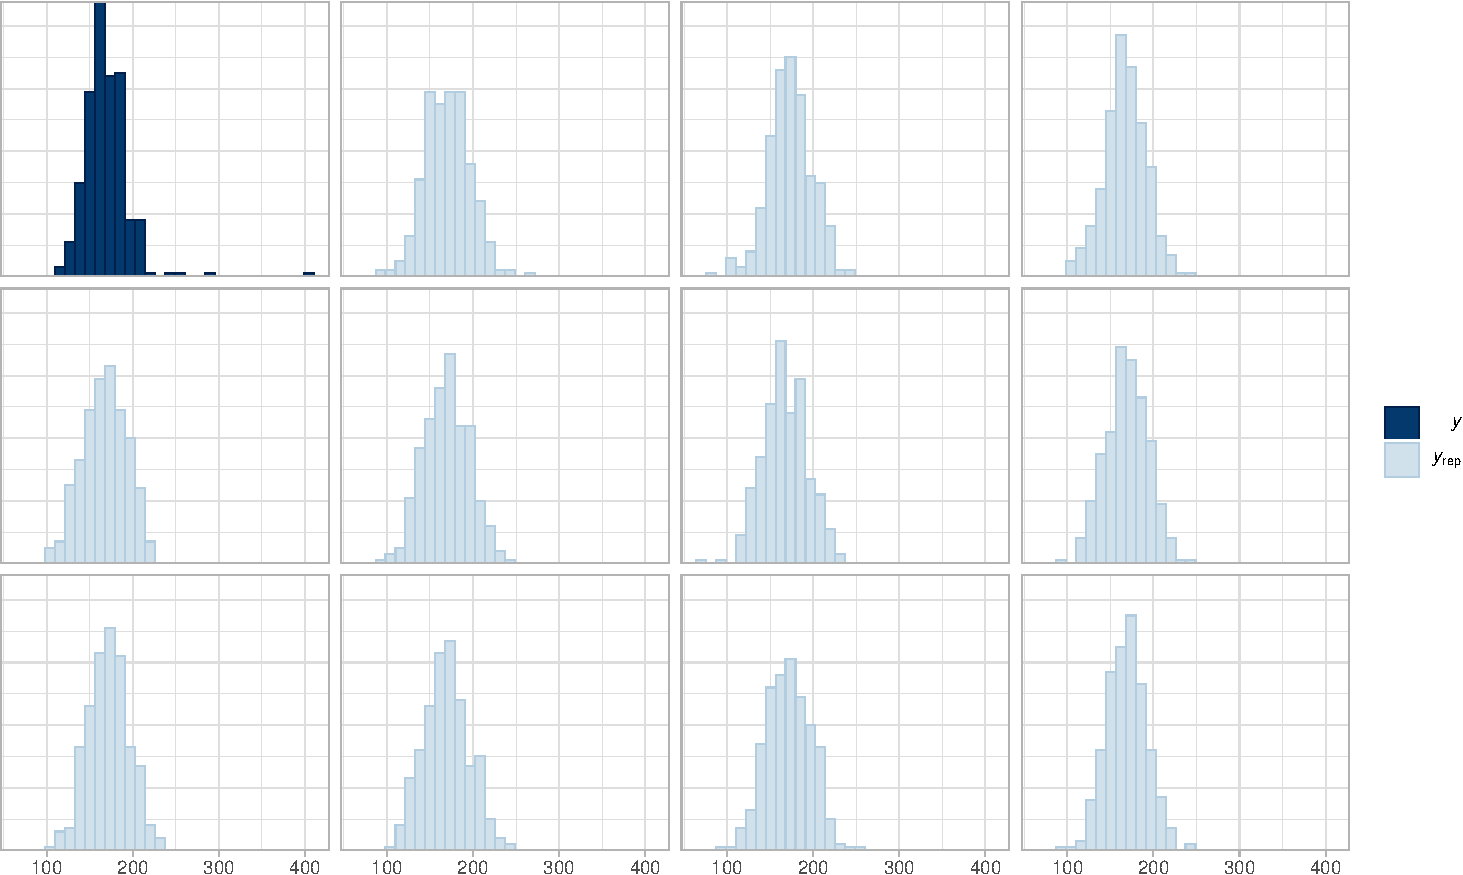
\includegraphics{03-compbayes-slides_files/figure-beamer/normalppc-1.pdf}
\caption{\label{fig:normalppc}Eleven samples from the posterior predictive distribution of the model \texttt{fit\_press}.}
\end{figure}

\normalsize

\end{frame}

\begin{frame}[fragile]



\small

\begin{Shaded}
\begin{Highlighting}[]
\KeywordTok{pp_check}\NormalTok{(fit_press, }\DataTypeTok{nsamples =} \DecValTok{100}\NormalTok{)}
\end{Highlighting}
\end{Shaded}

\begin{figure}
\centering
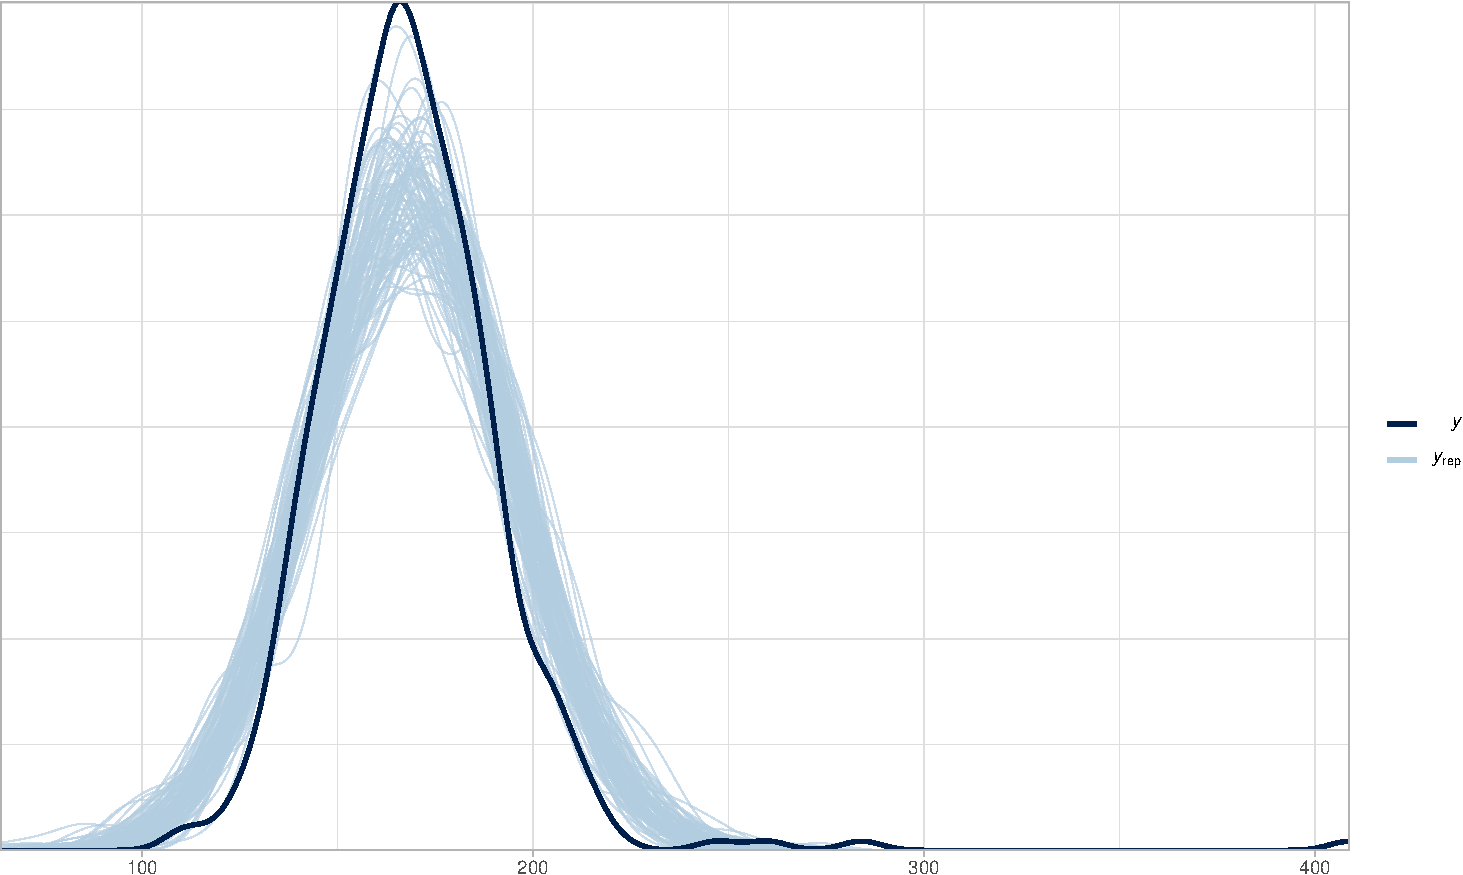
\includegraphics{03-compbayes-slides_files/figure-beamer/normalppc2-1.pdf}
\caption{\label{fig:normalppc2}Posterior predictive check that shows the fit of the model \texttt{fit\_press} in comparison to datasets from the posterior predictive distribution.}
\end{figure}

\normalsize

\end{frame}

\hypertarget{sec:lnfirst}{%
\section{Comparing different likelihoods: The log-normal likelihood}\label{sec:lnfirst}}

\begin{frame}

If \(y\) is log-normally distributed, this means that \(\log(y)\) is normally distributed.\footnote<.->{In fact, \(\log_e(y)\) or \(\ln(y)\), but we'll write it as just \(log()\)}

\begin{equation}
\begin{aligned}
\log(y) &\sim Normal( \mu, \sigma)\\
y &\sim \exp(Normal( \mu, \sigma)) \\
y &\sim LogNormal( \mu, \sigma)
\end{aligned}
\end{equation}

\color{red}

The log-normal distribution is again defined using \(\mu\) and \(\sigma\), but these correspond to the mean and standard deviation of the normally distributed logarithm of the data \(y\): \(\log(y)\).
\color{black}

\end{frame}

\begin{frame}{Re-fitting a single participant pressing a button repeatedly with a log-normal likelihood}
\protect\hypertarget{sec:lognormal}{}

\begin{block}{New likelihood:}

\begin{equation}
rt_n \sim LogNormal(\mu,\sigma)
\end{equation}

\end{block}

\begin{block}{New scale for the priors:}

\begin{equation}
\begin{aligned}
\mu &\sim Uniform(0, 8) \\
\sigma &\sim Uniform(0, 1) \\
\end{aligned}
\label{eq:logpriorsunif}
\end{equation}

\end{block}

\end{frame}

\begin{frame}

Because the parameters are in a different scale than the dependent variable, their interpretation changes:

\begin{itemize}
\tightlist
\item
  \emph{The location, \(\mu\)}: In our previous linear model, \(\mu\) represented the grand mean (or the grand median, or grand mode, since in a normal distribution the three coincide). But now, the grand mean is \(\exp(\mu +\sigma ^{2}/2)\) and the grand median is \(\exp(\mu)\). 
\item
  \emph{The scale, \(\sigma\)}: This is the standard deviation of the normal distribution of \(\log(y)\). The standard deviation of a log-normal distribution with \emph{location} \(\mu\) and \emph{shape} \(\sigma\) will be \(\exp(\mu +\sigma ^{2}/2)\times \sqrt(\exp(\sigma^2)- 1)\). 
\end{itemize}

\end{frame}

\begin{frame}[fragile]{Prior predictive distributions}
\protect\hypertarget{prior-predictive-distributions-1}{}

\small

\begin{Shaded}
\begin{Highlighting}[]
\NormalTok{N_samples <-}\StringTok{ }\DecValTok{1000}
\NormalTok{N_obs <-}\StringTok{ }\KeywordTok{nrow}\NormalTok{(df_noreading_data)}
\NormalTok{mu_samples <-}\StringTok{ }\KeywordTok{runif}\NormalTok{(N_samples, }\DecValTok{0}\NormalTok{, }\DecValTok{8}\NormalTok{)}
\NormalTok{sigma_samples <-}\StringTok{ }\KeywordTok{runif}\NormalTok{(N_samples, }\DecValTok{0}\NormalTok{, }\DecValTok{1}\NormalTok{)}
\NormalTok{prior_pred_ln <-}\StringTok{ }\KeywordTok{exp}\NormalTok{(}\KeywordTok{normal_predictive_distribution_fast}\NormalTok{(}
  \DataTypeTok{mu_samples =}\NormalTok{ mu_samples,}
  \DataTypeTok{sigma_samples =}\NormalTok{ sigma_samples,}
\NormalTok{  N_obs}
\NormalTok{))}
\end{Highlighting}
\end{Shaded}

\normalsize

\end{frame}

\begin{frame}[fragile]{Distribution of statistics}
\protect\hypertarget{distribution-of-statistics-1}{}

\scriptsize

\begin{Shaded}
\begin{Highlighting}[]
\NormalTok{(prior_pred_stat_ln <-}
\StringTok{  }\NormalTok{prior_pred_ln }\OperatorTok
\StringTok{  }\KeywordTok{group_by}\NormalTok{(iter) }\OperatorTok
\StringTok{  }\KeywordTok{summarize}\NormalTok{(}
    \DataTypeTok{min_rt =} \KeywordTok{min}\NormalTok{(rt_pred),}
    \DataTypeTok{max_rt =} \KeywordTok{max}\NormalTok{(rt_pred),}
    \DataTypeTok{average_rt =} \KeywordTok{mean}\NormalTok{(rt_pred),}
    \DataTypeTok{median_rt =} \KeywordTok{median}\NormalTok{(rt_pred)}
\NormalTok{  ) }\OperatorTok
\StringTok{  }\KeywordTok{pivot_longer}\NormalTok{(}\DataTypeTok{cols =} \KeywordTok{ends_with}\NormalTok{(}\StringTok{"rt"}\NormalTok{), }\DataTypeTok{names_to =} \StringTok{"stat"}\NormalTok{, }\DataTypeTok{values_to =} \StringTok{"rt"}\NormalTok{))}
\end{Highlighting}
\end{Shaded}

\begin{verbatim}
## # A tibble: 2,840 x 3
##    iter stat           rt
##   <dbl> <chr>       <dbl>
## 1  2.72 min_rt     106.  
## 2  2.72 max_rt     154.  
## 3  2.72 average_rt 130.  
## 4  2.72 median_rt  131.  
## 5  7.39 min_rt       2.99
## # ... with 2,835 more rows
\end{verbatim}

\normalsize

\end{frame}

\begin{frame}[fragile]

\vspace{.1in}



\scriptsize

\begin{Shaded}
\begin{Highlighting}[]
\NormalTok{prior_pred_stat_ln }\OperatorTok
\StringTok{  }\KeywordTok{ggplot}\NormalTok{(}\KeywordTok{aes}\NormalTok{(rt)) }\OperatorTok{+}
\StringTok{  }\KeywordTok{scale_x_continuous}\NormalTok{(}\StringTok{"Reaction times in ms"}\NormalTok{,}
    \DataTypeTok{trans =} \StringTok{"log"}\NormalTok{, }\DataTypeTok{breaks =} \KeywordTok{c}\NormalTok{(}\FloatTok{0.001}\NormalTok{, }\DecValTok{1}\NormalTok{, }\DecValTok{100}\NormalTok{, }\DecValTok{1000}\NormalTok{, }\DecValTok{10000}\NormalTok{, }\DecValTok{100000}\NormalTok{)) }\OperatorTok{+}
\StringTok{  }\KeywordTok{geom_histogram}\NormalTok{() }\OperatorTok{+}
\StringTok{  }\KeywordTok{facet_wrap}\NormalTok{(}\OperatorTok{~}\NormalTok{stat, }\DataTypeTok{ncol =} \DecValTok{1}\NormalTok{)}
\end{Highlighting}
\end{Shaded}

\begin{figure}
\centering
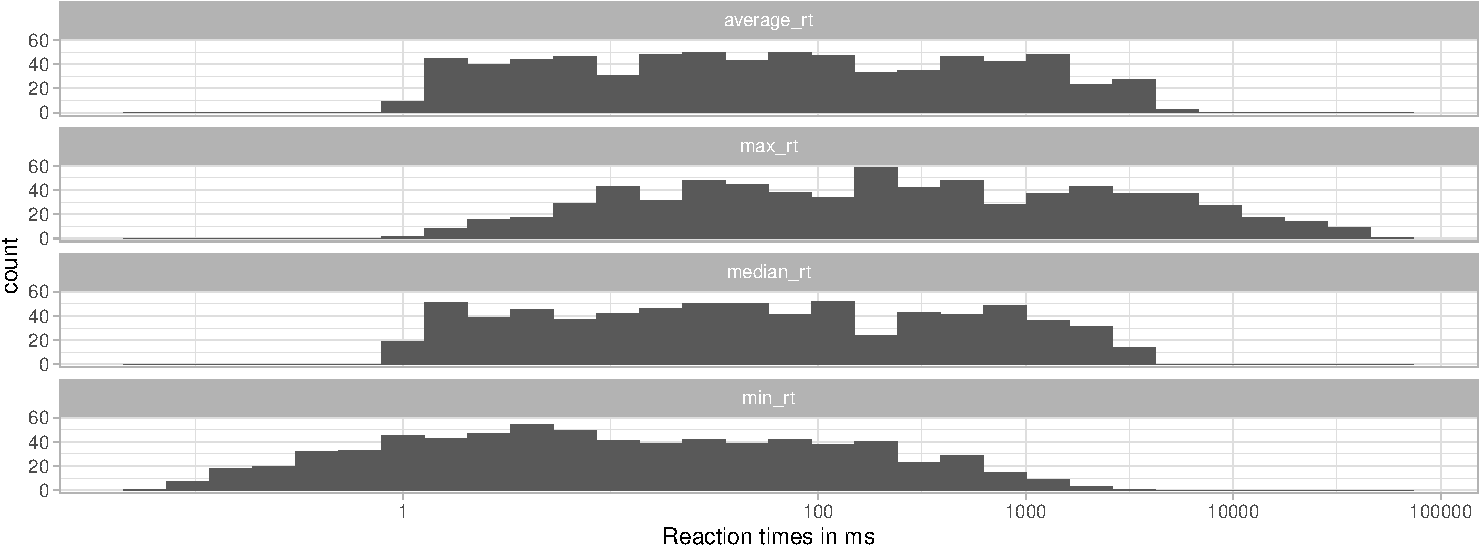
\includegraphics{03-compbayes-slides_files/figure-beamer/priorpredlogunif-1.pdf}
\caption{\label{fig:priorpredlogunif}Prior predictive distribution of averages, maximum, and minimum value of the log-normal model; the x-axis is log-transformed.}
\end{figure}

\normalsize

\textbf{We cannot not generate negative values anymore, since \(\exp(\)any number\() > 0\)}

\end{frame}

\begin{frame}{Better regularizing priors for the log-normal model}
\protect\hypertarget{better-regularizing-priors-for-the-log-normal-model}{}

\begin{equation}
rt_n \sim LogNormal(\mu,\sigma)
\end{equation}

\begin{equation}
\begin{aligned}
\mu &\sim Normal(6, 1.5) \\
\sigma &\sim Normal_+(0, 1) \\
\end{aligned}
\label{eq:logpriorsnorm}
\end{equation}

\end{frame}

\begin{frame}[fragile]

\begin{block}{Median effect for our new priors:}

\small

\begin{Shaded}
\begin{Highlighting}[]
\KeywordTok{c}\NormalTok{(}
  \DataTypeTok{lower =} \KeywordTok{exp}\NormalTok{(}\DecValTok{6} \OperatorTok{-}\StringTok{ }\DecValTok{2} \OperatorTok{*}\StringTok{ }\FloatTok{1.5}\NormalTok{),}
  \DataTypeTok{higher =} \KeywordTok{exp}\NormalTok{(}\DecValTok{6} \OperatorTok{+}\StringTok{ }\DecValTok{2} \OperatorTok{*}\StringTok{ }\FloatTok{1.5}\NormalTok{)}
\NormalTok{)}
\end{Highlighting}
\end{Shaded}

\begin{verbatim}
##  lower higher 
##     20   8103
\end{verbatim}

\normalsize

\end{block}

\end{frame}

\begin{frame}[fragile]{Prior predictive distributions}
\protect\hypertarget{prior-predictive-distributions-2}{}

\scriptsize

\begin{Shaded}
\begin{Highlighting}[]
\NormalTok{N_samples <-}\StringTok{ }\DecValTok{1000}
\NormalTok{N_obs <-}\StringTok{ }\KeywordTok{nrow}\NormalTok{(df_noreading_data)}
\NormalTok{mu_samples <-}\StringTok{ }\KeywordTok{rnorm}\NormalTok{(N_samples, }\DecValTok{6}\NormalTok{, }\FloatTok{1.5}\NormalTok{)}
\NormalTok{sigma_samples <-}\StringTok{ }\KeywordTok{rtnorm}\NormalTok{(N_samples, }\DecValTok{0}\NormalTok{, }\DecValTok{1}\NormalTok{, }\DataTypeTok{a =} \DecValTok{0}\NormalTok{)}
\NormalTok{(prior_pred_ln_better <-}\StringTok{ }\KeywordTok{exp}\NormalTok{(}\KeywordTok{normal_predictive_distribution_fast}\NormalTok{(}
  \DataTypeTok{mu_samples =}\NormalTok{ mu_samples,}
  \DataTypeTok{sigma_samples =}\NormalTok{ sigma_samples,}
\NormalTok{  N_obs}
\NormalTok{)))}
\end{Highlighting}
\end{Shaded}

\begin{verbatim}
## # A tibble: 361,000 x 3
##    iter trialn rt_pred
##   <dbl>  <dbl>   <dbl>
## 1  2.72   2.72    261.
## 2  2.72   7.39    248.
## 3  2.72  20.1     441.
## 4  2.72  54.6     841.
## 5  2.72 148.     2975.
## # ... with 3.61e+05 more rows
\end{verbatim}

\normalsize

\end{frame}

\begin{frame}[fragile]

\scriptsize

\begin{Shaded}
\begin{Highlighting}[]
\NormalTok{(prior_pred_stat_better_ln <-}\StringTok{ }\NormalTok{prior_pred_ln_better }\OperatorTok
\StringTok{  }\KeywordTok{group_by}\NormalTok{(iter) }\OperatorTok
\StringTok{  }\KeywordTok{summarize}\NormalTok{(}
    \DataTypeTok{min_rt =} \KeywordTok{min}\NormalTok{(rt_pred),}
    \DataTypeTok{max_rt =} \KeywordTok{max}\NormalTok{(rt_pred),}
    \DataTypeTok{average_rt =} \KeywordTok{mean}\NormalTok{(rt_pred),}
    \DataTypeTok{median_rt =} \KeywordTok{median}\NormalTok{(rt_pred)}
\NormalTok{  ) }\OperatorTok
\StringTok{  }\KeywordTok{pivot_longer}\NormalTok{(}
    \DataTypeTok{cols =} \KeywordTok{ends_with}\NormalTok{(}\StringTok{"rt"}\NormalTok{),}
    \DataTypeTok{names_to =} \StringTok{"stat"}\NormalTok{, }\DataTypeTok{values_to =} \StringTok{"rt"}
\NormalTok{  ))}
\end{Highlighting}
\end{Shaded}

\begin{verbatim}
## # A tibble: 2,840 x 3
##    iter stat            rt
##   <dbl> <chr>        <dbl>
## 1  2.72 min_rt        4.33
## 2  2.72 max_rt     9351.  
## 3  2.72 average_rt  734.  
## 4  2.72 median_rt   344.  
## 5  7.39 min_rt       23.8 
## # ... with 2,835 more rows
\end{verbatim}

\normalsize

\end{frame}

\begin{frame}[fragile]

\vspace{.1in}



\scriptsize

\begin{Shaded}
\begin{Highlighting}[]
\NormalTok{prior_pred_stat_better_ln }\OperatorTok\StringTok{ }\KeywordTok{ggplot}\NormalTok{(}\KeywordTok{aes}\NormalTok{(rt)) }\OperatorTok{+}
\StringTok{    }\KeywordTok{scale_x_continuous}\NormalTok{(}\DataTypeTok{trans =} \StringTok{"log"}\NormalTok{,}
                       \DataTypeTok{breaks =} \KeywordTok{c}\NormalTok{(}\FloatTok{0.001}\NormalTok{, }\DecValTok{1}\NormalTok{, }\DecValTok{100}\NormalTok{, }\DecValTok{1000}\NormalTok{, }\DecValTok{10000}\NormalTok{, }\DecValTok{100000}\NormalTok{)) }\OperatorTok{+}
\StringTok{    }\KeywordTok{geom_histogram}\NormalTok{() }\OperatorTok{+}
\StringTok{    }\KeywordTok{facet_wrap}\NormalTok{(}\OperatorTok{~}\NormalTok{stat, }\DataTypeTok{ncol =} \DecValTok{1}\NormalTok{) }\OperatorTok{+}
\StringTok{    }\KeywordTok{coord_cartesian}\NormalTok{(}\DataTypeTok{xlim =} \KeywordTok{c}\NormalTok{(}\FloatTok{0.001}\NormalTok{, }\DecValTok{300000}\NormalTok{))}
\end{Highlighting}
\end{Shaded}

\begin{figure}
\centering
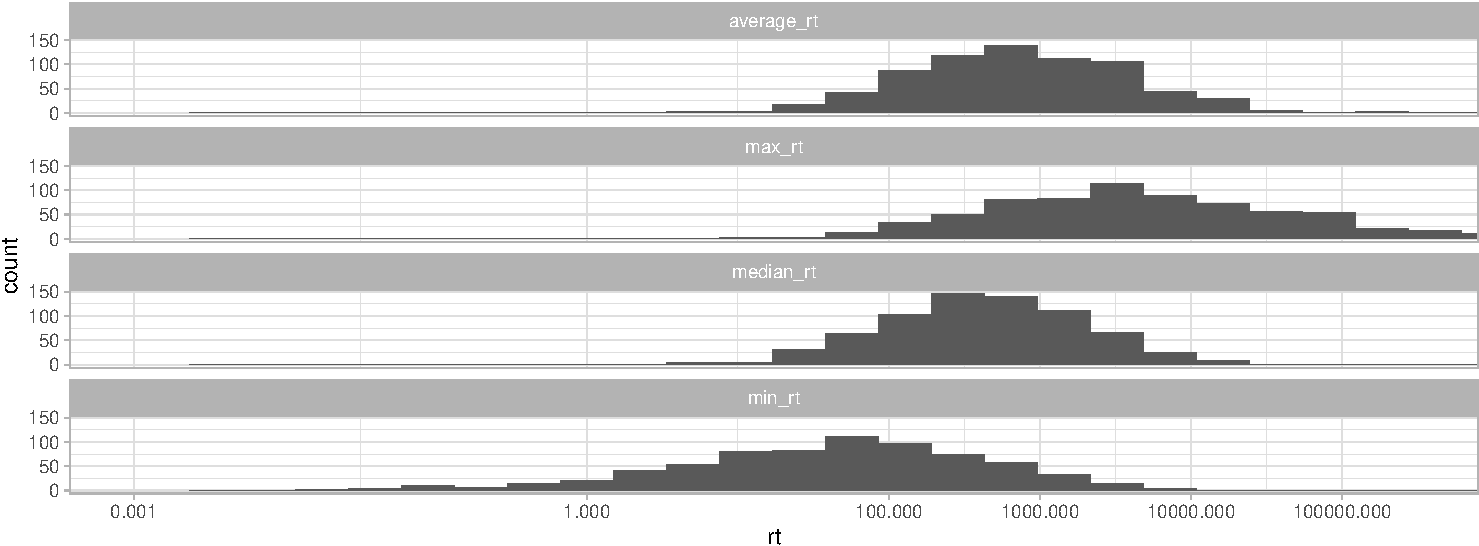
\includegraphics{03-compbayes-slides_files/figure-beamer/priorpredlognorm-1.pdf}
\caption{\label{fig:priorpredlognorm}Prior predictive distribution of averages, maximum, and minimum value of the log-normal model with better priors.}
\end{figure}

\normalsize

\end{frame}

\begin{frame}[fragile]

\begin{block}{brms model with reasonable priors:\footnote<.->{Notice that we need to specify that the family is \texttt{lognormal()}}}

\small

\begin{Shaded}
\begin{Highlighting}[]
\NormalTok{fit_press_ln <-}\StringTok{ }\KeywordTok{brm}\NormalTok{(rt }\OperatorTok{~}\StringTok{ }\DecValTok{1}\NormalTok{,}
  \DataTypeTok{data =}\NormalTok{ df_noreading_data,}
  \DataTypeTok{family =} \KeywordTok{lognormal}\NormalTok{(),}
  \DataTypeTok{prior =} \KeywordTok{c}\NormalTok{(}
    \KeywordTok{prior}\NormalTok{(}\KeywordTok{normal}\NormalTok{(}\DecValTok{6}\NormalTok{, }\FloatTok{1.5}\NormalTok{), }\DataTypeTok{class =}\NormalTok{ Intercept),}
    \KeywordTok{prior}\NormalTok{(}\KeywordTok{normal}\NormalTok{(}\DecValTok{0}\NormalTok{, }\DecValTok{1}\NormalTok{), }\DataTypeTok{class =}\NormalTok{ sigma)}
\NormalTok{  )}
\NormalTok{)}
\end{Highlighting}
\end{Shaded}

\normalsize

\end{block}

\end{frame}

\begin{frame}[fragile]

\scriptsize

\begin{Shaded}
\begin{Highlighting}[]
\NormalTok{fit_press_ln}
\end{Highlighting}
\end{Shaded}

\begin{verbatim}
##  Family: lognormal 
##   Links: mu = identity; sigma = identity 
## Formula: rt ~ 1 
##    Data: df_noreading_data (Number of observations: 361) 
## Samples: 4 chains, each with iter = 2000; warmup = 1000; thin = 1;
##          total post-warmup samples = 4000
## 
## Population-Level Effects: 
##           Estimate Est.Error l-95% CI u-95% CI Rhat
## Intercept     5.12      0.01     5.10     5.13 1.00
##           Bulk_ESS Tail_ESS
## Intercept     3976     2869
## 
## Family Specific Parameters: 
##       Estimate Est.Error l-95% CI u-95% CI Rhat
## sigma     0.13      0.01     0.13     0.15 1.00
##       Bulk_ESS Tail_ESS
## sigma     3362     2436
## 
## Samples were drawn using sampling(NUTS). For each parameter, Bulk_ESS
## and Tail_ESS are effective sample size measures, and Rhat is the potential
## scale reduction factor on split chains (at convergence, Rhat = 1).
\end{verbatim}

\normalsize

\end{frame}

\begin{frame}[fragile]

\begin{block}{How long does it take to press the space bar in milliseconds?}

\scriptsize

\begin{Shaded}
\begin{Highlighting}[]
\NormalTok{estimate_ms <-}\StringTok{ }\KeywordTok{exp}\NormalTok{(}\KeywordTok{posterior_samples}\NormalTok{(fit_press_ln)}\OperatorTok{$}\NormalTok{b_Intercept)}
\KeywordTok{c}\NormalTok{(}\DataTypeTok{mean =} \KeywordTok{mean}\NormalTok{(estimate_ms), }\KeywordTok{quantile}\NormalTok{(estimate_ms, }\DataTypeTok{probs =} \KeywordTok{c}\NormalTok{(.}\DecValTok{025}\NormalTok{, }\FloatTok{.975}\NormalTok{)))}
\end{Highlighting}
\end{Shaded}

\begin{verbatim}
## mean 2.5%  98% 
##  167  165  169
\end{verbatim}

\normalsize

\end{block}

\end{frame}

\begin{frame}[fragile]{Posterior predictive checks}
\protect\hypertarget{posterior-predictive-checks}{}



\small

\begin{Shaded}
\begin{Highlighting}[]
\KeywordTok{pp_check}\NormalTok{(fit_press_ln, }\DataTypeTok{nsamples =} \DecValTok{100}\NormalTok{)}
\end{Highlighting}
\end{Shaded}

\begin{figure}
\centering
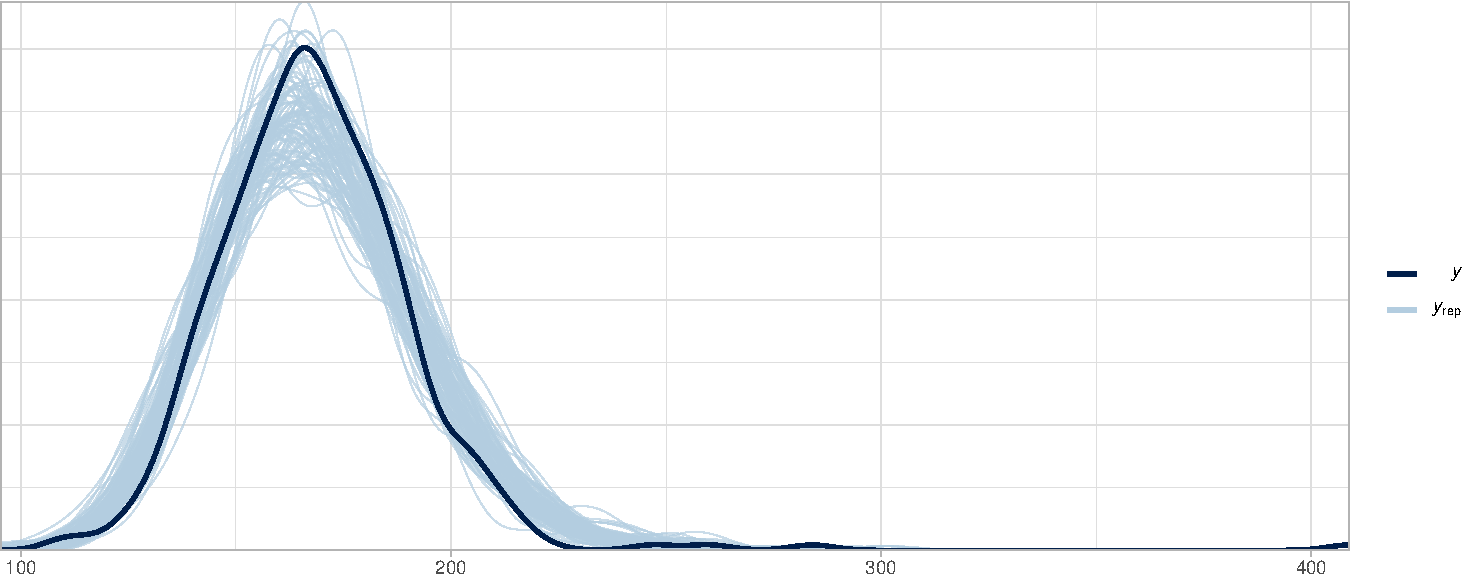
\includegraphics{03-compbayes-slides_files/figure-beamer/lognppc-1.pdf}
\caption{\label{fig:lognppc}Posterior predictive distribution of \texttt{fit\_noreading\_ln}}
\end{figure}

\normalsize

\end{frame}

\begin{frame}

\begin{block}{\emph{Are the posterior predicted data now more similar to the real data, compared to the case where we had a Normal likelihood?}}

\vspace{.1in}

We suspect that the normal distribution would generate reaction times that are too fast (since it's symmetrical) and that the log-normal distribution may capture the long tail better than the normal model.

\end{block}

\end{frame}

\begin{frame}[fragile]

\vspace{.1in}

\scriptsize

\begin{Shaded}
\begin{Highlighting}[]
\KeywordTok{pp_check}\NormalTok{(fit_press, }\DataTypeTok{type =} \StringTok{"stat"}\NormalTok{, }\DataTypeTok{stat =} \StringTok{"min"}\NormalTok{) }\OperatorTok{+}
\StringTok{  }\KeywordTok{ggtitle}\NormalTok{(}\StringTok{"Normal model"}\NormalTok{)}
\KeywordTok{pp_check}\NormalTok{(fit_press_ln, }\DataTypeTok{type =} \StringTok{"stat"}\NormalTok{, }\DataTypeTok{stat =} \StringTok{"min"}\NormalTok{) }\OperatorTok{+}
\StringTok{  }\KeywordTok{ggtitle}\NormalTok{(}\StringTok{"Log-normal model"}\NormalTok{)}
\end{Highlighting}
\end{Shaded}

\begin{figure}
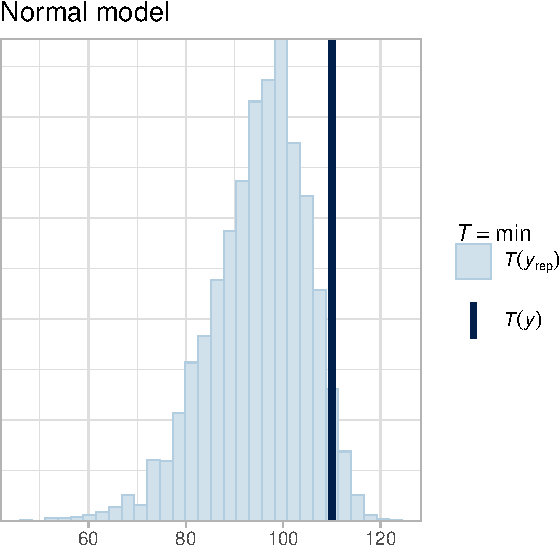
\includegraphics[width=0.45\linewidth]{03-compbayes-slides_files/figure-beamer/ppcheckmin-1} 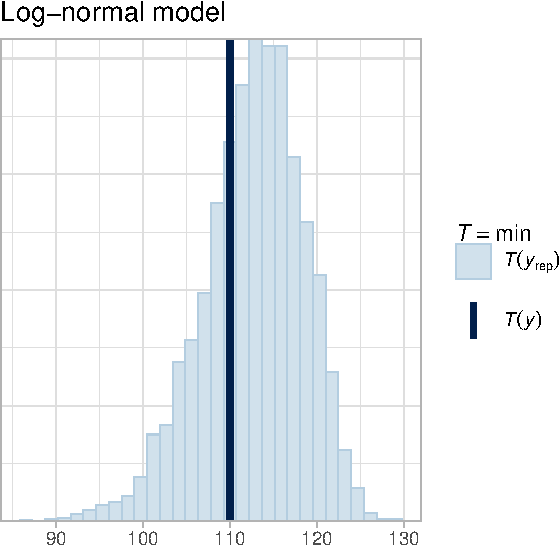
\includegraphics[width=0.45\linewidth]{03-compbayes-slides_files/figure-beamer/ppcheckmin-2} \caption{Distribution of minimum values in a posterior predictive check. The minimum in the data is 110 ms.}\label{fig:ppcheckmin}
\end{figure}

\normalsize

\end{frame}

\begin{frame}[fragile]

\vspace{.1in}

\scriptsize

\begin{Shaded}
\begin{Highlighting}[]
\KeywordTok{pp_check}\NormalTok{(fit_press, }\DataTypeTok{type =} \StringTok{"stat"}\NormalTok{, }\DataTypeTok{stat =} \StringTok{"max"}\NormalTok{) }\OperatorTok{+}
\StringTok{  }\KeywordTok{ggtitle}\NormalTok{(}\StringTok{"Normal model"}\NormalTok{)}
\KeywordTok{pp_check}\NormalTok{(fit_press_ln, }\DataTypeTok{type =} \StringTok{"stat"}\NormalTok{, }\DataTypeTok{stat =} \StringTok{"max"}\NormalTok{) }\OperatorTok{+}
\StringTok{  }\KeywordTok{ggtitle}\NormalTok{(}\StringTok{"Log-normal model"}\NormalTok{)}
\end{Highlighting}
\end{Shaded}

\begin{figure}
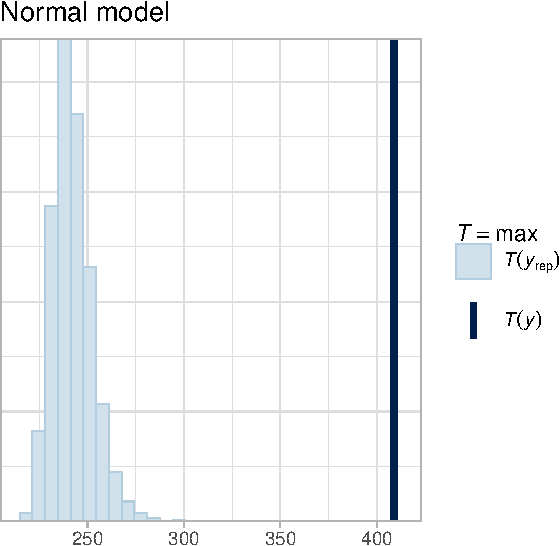
\includegraphics[width=0.45\linewidth]{03-compbayes-slides_files/figure-beamer/ppcheckmax-1} 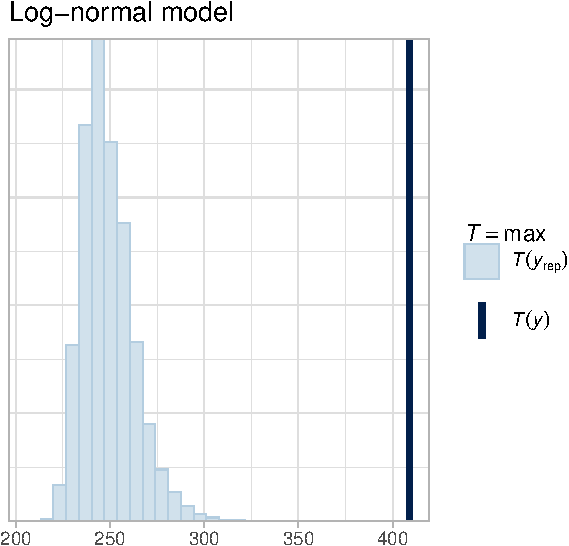
\includegraphics[width=0.45\linewidth]{03-compbayes-slides_files/figure-beamer/ppcheckmax-2} \caption{Distribution of maximum values in a posterior predictive check. The maximum in the data is 409 ms.}\label{fig:ppcheckmax}
\end{figure}

\normalsize

\end{frame}

\begin{frame}[fragile]

\begin{block}{\color{blue} Exercises}

3.8.3.1 Generate posterior predictive distributions based on the previous model (3.8.2.1) and plot them.

3.8.3.2 For the log-normal model \texttt{fit\_press\_ln}, change the prior of \(\sigma\) so that it is a lognormal distribution with location (\(\mu\)) of \(-2\) and scale (\(\sigma\)) of \(.5\). What is the meaning of this prior? Is it a good prior? Generate and plot prior predictive distributions. Do the new estimates change when you fit the model?

3.8.3.3 For the log-normal model, what is the mean (rather than median) time that takes to press the space bar, what is the standard deviation of the reaction times in milliseconds?

\ldots{}.

\end{block}

\end{frame}

\begin{frame}[fragile]

3.8.3.4 Would it make sense to use a ``skew normal distribution'' instead of the lognormal? The skew normal distribution has three parameters location \(\xi\), scale \(\omega\), and shape \(\alpha\). The distribution is right skewed if \(\alpha >0\), is left skewed if \(\alpha <0\), and is identical to the regular normal distribution if \(\alpha =0\). For fitting this in \texttt{brms}, one needs to change \texttt{family} and set it to \texttt{skew\_normal()}, and add a prior of \texttt{class\ =\ alpha} (location remains \texttt{class\ =\ Intercept} and scale, \texttt{class\ =\ sigma}).

\begin{itemize}
\item
  Fit this model with a prior that assigns approximately 95\% of the prior probability mass of \texttt{alpha} to be between 0 and 10.
\item
  Generate posterior predictive distributions and compare the posterior distribution of summary statistics of the skew normal with the normal and log-normal
\end{itemize}

\end{frame}

\begin{frame}{What did we do?}
\protect\hypertarget{what-did-we-do}{}

\begin{itemize}
\tightlist
\item
  fitted and interpreted a normal model
\item
  looked at the effect of priors:

  \begin{itemize}
  \tightlist
  \item
    prior predictive distributions
  \item
    sensitivity analysis
  \end{itemize}
\item
  looked at the fit of the posterior:

  \begin{itemize}
  \tightlist
  \item
    posterior predictive distribution (descriptive adequacy)
  \end{itemize}
\item
  fitted and interpreted a log-normal model
\item
  compared a normal model with a log-normal one
\end{itemize}

\end{frame}

\begin{frame}{References}
\protect\hypertarget{references}{}

\hypertarget{refs}{}
\leavevmode\hypertarget{ref-R-brms}{}%
Bürkner, Paul-Christian. 2019. \emph{Brms: Bayesian Regression Models Using 'Stan'}. \url{https://CRAN.R-project.org/package=brms}.

\leavevmode\hypertarget{ref-carpenter2017stan}{}%
Carpenter, Bob, Andrew Gelman, Matthew D Hoffman, Daniel Lee, Ben Goodrich, Michael Betancourt, Marcus Brubaker, Jiqiang Guo, Peter Li, and Allen Riddell. 2017. ``Stan: A Probabilistic Programming Language.'' \emph{Journal of Statistical Software} 76 (1). Columbia Univ., New York, NY (United States); Harvard Univ., Cambridge, MA (United States).

\leavevmode\hypertarget{ref-rstanarm}{}%
Goodrich, Ben, Jonah Gabry, Imad Ali, and Sam Brilleman. 2018. ``Rstanarm: Bayesian Applied Regression Modeling via Stan.'' \url{http://mc-stan.org/}.

\leavevmode\hypertarget{ref-lunn2000winbugs}{}%
Lunn, D.J., A. Thomas, N. Best, and D. Spiegelhalter. 2000. ``WinBUGS-A Bayesian Modelling Framework: Concepts, Structure, and Extensibility.'' \emph{Statistics and Computing} 10 (4). Springer: 325--37.

\leavevmode\hypertarget{ref-plummer2016jags}{}%
Plummer, Martin. 2016. ``JAGS Version 4.2.0 User Manual.''

\leavevmode\hypertarget{ref-Salvatier2016}{}%
Salvatier, John, Thomas V. Wiecki, and Christopher Fonnesbeck. 2016. ``Probabilistic Programming in Python Using PyMC3.'' \emph{PeerJ Computer Science} 2 (April). PeerJ: e55. \url{https://doi.org/10.7717/peerj-cs.55}.

\leavevmode\hypertarget{ref-vasishthProcessingChineseRelative2013}{}%
Vasishth, Shravan, Zhong Chen, Qiang Li, and Gueilan Guo. 2013. ``Processing Chinese Relative Clauses: Evidence for the Subject--Relative Advantage.'' \emph{PLOS ONE} 8 (10): e77006. \url{https://doi.org/10.1371/journal.pone.0077006}.

\end{frame}

\end{document}
